\documentclass[11pt]{article}
\usepackage[a4paper,margin=2.5cm]{geometry}
\usepackage{amsmath,amssymb}
\usepackage{graphicx}
\usepackage{booktabs}
\usepackage{longtable}
\usepackage{array}
\usepackage{hyperref}
\usepackage{enumitem}
\usepackage{xcolor}
\usepackage{caption}
\usepackage{microtype}
\sloppy
\graphicspath{{figures/}}
\setlist[itemize]{leftmargin=1.2em}
\setlist[enumerate]{leftmargin=1.4em}
\renewcommand{\arraystretch}{1.15}

\title{BOAMP M0 Procurement Recurrence Linking\\
\large Detailed Technical Reference for Data Audit, Preprocessing, Recurrence-Linking
Algorithm, and Survival Analysis}
\author{Gigalis Predictive-Modeling Internship --- Current Independent Study}
\date{Repository state of July 2026 (outputs last regenerated 2026-07-15 via the
notebook front-ends; key datasets byte-identical to the audited 2026-07-13
script run)}

\begin{document}
\maketitle

\begin{abstract}
This report is the detailed technical reference for the current BOAMP-only
procurement recurrence-linking pipeline covering digital/ICT public
contracts in Pays de la Loire, 2015--2026. It documents the concrete
implementation choices, data audit, preprocessing rules, the deterministic
M0 recurrence-linking algorithm, intermediate diagnostics, and
survival-modeling outputs, in a form that can be checked, reproduced, and
handed off. BOAMP notices carry no field identifying whether a call for
tenders (\emph{appel d'offre}) is a recurrence of an earlier contract for the
same buyer; the relationship must be inferred from observable signals:
buyer identity, free-text object similarity, CPV classification, and timing
relative to the source contract's estimated end date.

Starting from 84{,}623 cleaned BOAMP notices published for Pays de la Loire
buyers between 2015-03-02 and 2026-07-13, the pipeline identifies 3{,}159
digital/ICT \texttt{APPEL\_OFFRE} source notices. A deterministic
four-component scoring rule (text, CPV, timing, buyer-key reliability) is
applied to 6{,}137 blocked candidate pairs; at the reference (``balanced'')
threshold this yields 618 linked proxy-recurrence events, an event rate of
19.6\%. The official survival handoff,
\texttt{boamp\_survival\_m0\_balanced.csv}, contains one row per eligible
source notice with a binary \texttt{event} indicator and an observed
\texttt{time\_to\_event\_or\_censor\_months} survival time.

Kaplan--Meier survival never crosses 50\% under the reference definition
(median survival is undefined; restricted mean survival time at 60 months is
53.5 months), reflecting 80.4\% censoring. A buyer-clustered Cox model finds
a statistically significant negative association between the duration-imputation
flag and the recurrence hazard (HR $=0.433$, $p<0.001$), while the effect of
declared duration itself is small and not significant in the reference
design (HR $=0.923$, $p=0.38$). A dedicated duration-leakage audit shows
this duration effect is \emph{not} robust: it reverses sign (HR $=1.344$)
under an alternative linkage design that does not center candidate search on
declared duration, indicating that duration-related survival findings are
conditional on the current temporal-blocking design rather than independent
substantive effects. Blocking coverage is a first-order limitation: only
39.1\% of eligible sources have at least one scored candidate. The reference
event set should therefore be read as a \emph{proxy recurrence signal}
constructed under a fully documented, auditable rule --- not as a verified
renewal probability.
\end{abstract}

\section*{How to read this report}
This document is the single, comprehensive technical reference for the
current repository state. It is organized the way a handoff document should
be: Section~\ref{sec:scope} gives the business framing, the objectives, and
the research questions; Section~\ref{sec:workflow} documents the
computational workflow and run flow as they actually exist in the
repository, including where implementation is duplicated between scripts
and notebooks; Sections \ref{sec:data}--\ref{sec:dq} document the raw data
and its quality; Sections \ref{sec:pipeline}--\ref{sec:output} document
preprocessing and the M0 linking algorithm mechanically, with a full worked
example in Section~\ref{sec:worked}; Section~\ref{sec:reliability}
consolidates the credibility diagnostics (blocking coverage, score margins,
an unsupervised Fellegi--Sunter precision/recall estimate,
corruption-recovery robustness); Sections
\ref{sec:survival-methods}--\ref{sec:sensitivity} document the survival
analysis, its methods, results, and robustness under alternative event
definitions; Section~\ref{sec:status} classifies every method by its
implementation status (verified / pending validation / partial / deferred /
proposed); Section~\ref{sec:conclusions} states plainly what is and is not
supported by the current evidence. All figures and tables reflect the
current repository run; every number quoted here is reproduced in a
machine-readable CSV under \texttt{reports/tables/} or
\texttt{data/processed/}, referenced inline.

\paragraph{Relationship to the other documents in \texttt{reports/}.}
This report is the master reference and subsumes the others.
\texttt{boamp\_m0\_preprocessing\_report.md} is the standalone
data-retrieval and preprocessing report (Sections
\ref{sec:data}--\ref{sec:pipeline} here, in more operational detail);
\texttt{linkage\_quality\_evaluation.tex/.pdf} is the focused
credibility-audit companion (Sections
\ref{sec:diagnostics}--\ref{sec:sensitivity} here);
\texttt{credibility\_audit\_report.md} is its short machine-checkable
executive summary; \texttt{run\_logs/run\_log.md} is the append-only
execution history. Where documents overlap, they were checked for numerical
consistency against the same generated tables; no document reports a value
the others contradict.

\paragraph{Epistemic labeling convention.} Throughout, claims are separated
into four kinds: (i) \emph{literature-standard} methods, cited to their
sources in the bibliography; (ii) \emph{project-specific methodological
choices} (e.g.\ score weights, threshold percentiles), which are documented
decisions, not fitted or externally justified quantities; (iii)
\emph{data- or compute-constrained} choices (e.g.\ TF-IDF instead of
transformer embeddings, the Pays-de-la-Loire re-scoping), where the
constraint is stated; and (iv) \emph{proposed improvements}, which are not
implemented and are listed only in Sections \ref{sec:status} and
\ref{sec:repro}.

\tableofcontents

\section{Project Scope}
\label{sec:scope}

\subsection{Business Context}
Gigalis manages a portfolio of public digital-infrastructure contracts in
the Pays de la Loire region. A recurring operational question is: \emph{when
is a given procurement contract likely to be re-tendered?} Anticipating this
lets account managers prepare competitive offers ahead of a renewal
campaign instead of discovering a re-tender after the fact.

\subsection{Why BOAMP?}
The \emph{Bulletin Officiel des Annonces de March\'es Publics} (BOAMP) is
the official French public-procurement gazette. Contracts above the
relevant thresholds must be published there, across the notice lifecycle:
pre-information, call for tenders (\texttt{APPEL\_OFFRE}), award
(\texttt{ATTRIBUTION}), and correction/modification notices.

\subsection{Core Problem}
BOAMP does not provide an explicit field linking an original call for
tenders to its later recurrence. Each notice is a standalone publication
event. The recurrence relationship must be \textbf{inferred} from a
combination of signals: the same buyer re-issuing a broadly similar
procurement need in the time window around when the original contract was
expected to end.

\subsection{Scope of the Current Study}
This is a fresh, independent pipeline; it does not reuse or compare against
any prior BOAMP study, report, or event count. It targets a specific,
documented scope bundle:
\begin{itemize}
  \item \textbf{Period}: 2015-01-01 to 2026-07-13 (latest available). The
  BOAMP Opendatasoft corpus itself begins 2015-03-02, so January--February
  2015 contribute no notices by construction, not by retrieval failure.
  \item \textbf{Geography}: Pays de la Loire only --- buyer department code
  in $\{44,49,53,72,85\}$ (Loire-Atlantique, Maine-et-Loire, Mayenne,
  Sarthe, Vend\'ee), applied \textbf{server-side} at retrieval time via the
  API's \texttt{where} clause.
  \item \textbf{Theme}: digital/ICT contracts --- CPV divisions
  $\{32,35,48,72\}$ (telecommunications equipment, security, software, IT
  services) and their subcategories, applied as a \textbf{hard filter} when
  constructing the M0 source population (Section~\ref{sec:pipeline}).
\end{itemize}
No external SIREN/SIRET enrichment is performed anywhere in this pipeline:
no INSEE SIRENE API call, no data.gouv.fr entreprise search, no external
company database. Every identifier used is a BOAMP-provided value that is
only format/checksum-validated, never looked up or inferred externally
(Section~\ref{sec:buyerkey}).

\subsection{Objectives and Research Questions}
\label{sec:rq}
The study's operational objective is a documented, reproducible,
BOAMP-only pipeline that turns raw procurement notices into a
contract-level survival dataset suitable for time-to-recurrence modeling.
The research questions actually addressed by the current implementation
are:
\begin{enumerate}
  \item[\textbf{RQ1.}] \emph{Can recurrence of a procurement need be
  operationalized from BOAMP alone?} --- i.e.\ can a transparent,
  deterministic rule link an initial call for tenders to a plausible later
  re-tender by the same buyer, without external enrichment or supervised
  learning? (Sections \ref{sec:pipeline}--\ref{sec:output}.)
  \item[\textbf{RQ2.}] \emph{How reliable are the BOAMP fields the rule
  depends on} --- buyer identifiers, CPV codes, and especially the declared
  contract duration? This includes the internship guide's Week-1
  ``scientific question'' on duration-field reliability.
  (Sections \ref{sec:data}--\ref{sec:dq}.)
  \item[\textbf{RQ3.}] \emph{What does the time-to-recurrence distribution
  of the constructed proxy event look like}, and which observable covariates
  associate with the recurrence hazard? (Sections
  \ref{sec:survival-methods}--\ref{sec:results}.)
  \item[\textbf{RQ4.}] \emph{How credible and how stable are these
  answers} under internal diagnostics (model-based precision/recall,
  corruption stress tests) and under perturbations of the event definition
  itself (thresholds, temporal windows, duration-independent designs)?
  (Sections \ref{sec:reliability}, \ref{sec:sensitivity}.)
\end{enumerate}
The short answers, defended in the body of the report, are: RQ1 --- yes,
mechanically, but only as a \emph{proxy} signal whose external accuracy is
unmeasured; RQ2 --- buyer identifiers and durations are weak (72.8\%
name-fallback keys; 88.0\% imputed durations), CPV is moderate and decaying
in recent years; RQ3 --- the proxy recurrence is a slow event (median
survival undefined; RMST$_{60}$ = 53.5 months) whose strongest apparent
covariate effects are entangled with the linkage design; RQ4 --- internally
coherent but materially sensitive to the temporal design, with a
demonstrated duration-circularity artifact that is the report's
highest-priority caveat.

\section{Computational Workflow and Run Flow}
\label{sec:workflow}

\subsection{Observed Pipeline Structure}
The repository implements a linear data pipeline followed by a fan-out of
evaluation analyses. The persisted datasets and their producer scripts are
inventoried in Table~\ref{tab:lineage} (Section~\ref{sec:construction});
the execution order, reconstructed from script input/output declarations
and \texttt{reports/tables/audit\_data\_lineage.csv}, is:
\begin{enumerate}
  \item \textbf{Retrieval} (\texttt{scripts/download\_boamp.py}): DILA
  Opendatasoft API $\rightarrow$ \texttt{data/raw/boamp/pdl/boamp\_YYYYMM.json}
  (139 monthly files + a download manifest; raw files are never
  overwritten).
  \item \textbf{Flattening} (\texttt{scripts/parse\_boamp.py}): raw JSON
  $\rightarrow$ \texttt{data/interim/boamp\_raw\_flattened.csv} (84{,}623
  notices $\times$ 42 columns), via the adaptive schema extractor in
  \texttt{src/utils/boamp\_schema.py}.
  \item \textbf{Preprocessing} (notebook \texttt{05} / script
  \texttt{preprocess\_boamp\_m0.py}): cleaned notice table
  (\texttt{boamp\_clean\_m0\_no\_enrichment.csv}, 93 columns) and the
  digital-scope source population (\texttt{boamp\_m0\_sources.csv},
  3{,}159 rows).
  \item \textbf{Candidate generation and scoring} (notebook \texttt{07} /
  script \texttt{build\_m0\_candidate\_pairs.py}): blocked, scored pairs
  (\texttt{boamp\_m0\_candidate\_pairs.csv}, 6{,}137 rows).
  \item \textbf{Linkage and survival handoff} (notebook \texttt{08} /
  script \texttt{run\_m0\_linkage.py}): broad/balanced/strict link files
  and the reference survival dataset
  (\texttt{boamp\_survival\_m0\_balanced.csv}), plus the
  \texttt{m0\_*.csv} quality tables.
  \item \textbf{Evaluation fan-out} (consumes stages 3--5, never mutates
  them): repository audit (\texttt{audit\_current\_project.py} / notebook
  \texttt{13}), Fellegi--Sunter mixture (notebook \texttt{11} / script
  \texttt{eval\_m3\_*}), corruption recovery (notebook \texttt{12} /
  \texttt{eval\_m4\_*}), threshold/ablation/variant-KM sensitivity
  (\texttt{eval\_m6a/b/c\_*}, script-only), temporal-window sensitivity
  (notebook \texttt{14} / \texttt{eval\_m6d\_*}), duration leakage
  (notebook \texttt{15} / \texttt{eval\_duration\_leakage.py}), and the
  survival analysis (notebook \texttt{16} /
  \texttt{run\_survival\_analysis.py}). Sensitivity runs write their own
  link/survival datasets (\texttt{boamp\_m0\_links\_window\_*m.csv},
  \texttt{boamp\_survival\_m0\_*.csv}) --- these are sensitivity artifacts,
  not replacements for the balanced reference handoff.
  \item \textbf{Reporting utilities}: \texttt{make\_figures.py},
  \texttt{make\_evaluation\_figures.py}, \texttt{make\_report\_figures.py}
  (figures 01--18), and the report-assembly helpers
  \texttt{\_build\_schema\_summary.py}, \texttt{\_build\_source\_trace.py},
  \texttt{\_build\_final\_audit.py}.
\end{enumerate}

\subsection{Dual Script/Notebook Implementation --- Observed State}
\label{sec:dualimpl}
The pipeline exists in two forms, and the relationship between them is not
uniform. This is reported as observed, not idealized:
\begin{itemize}
  \item \textbf{Stages 3--5 are implemented twice.} Notebooks
  \texttt{05}/\texttt{07}/\texttt{08} contain the preprocessing, candidate
  generation, and linkage logic \emph{inline} (they do not import the
  scripts), while scripts \texttt{preprocess\_boamp\_m0.py},
  \texttt{build\_m0\_candidate\_pairs.py}, and \texttt{run\_m0\_linkage.py}
  implement the same logic as a headless batch backend. Both write the same
  official output files. The duplication is a maintenance risk (a rule
  changed in one place could silently diverge from the other), but as of
  the current run the two implementations are \emph{verified equivalent in
  output}: the 2026-07-15 notebook regeneration reproduced the audited
  2026-07-13 script outputs byte-for-byte (SHA-256 of
  \texttt{boamp\_m0\_sources.csv}, \texttt{boamp\_m0\_candidate\_pairs.csv},
  and \texttt{boamp\_survival\_m0\_balanced.csv} match
  \texttt{reports/tables/audit\_dataset\_inventory.csv} exactly).
  \item \textbf{Stage-6 notebooks 14 and 15 share code with the scripts.}
  They \texttt{import build\_m0\_candidate\_pairs} and
  \texttt{run\_m0\_linkage} from \texttt{scripts/}, so the M0 scoring rule
  used in the temporal-window and duration-leakage sensitivity analyses has
  a single definition.
  \item \textbf{Notebooks 11, 12, and 16 are inline analyses} (no script
  import); notebook \texttt{13} is the only remaining thin viewer, with a
  \texttt{RUN\_SCRIPT} toggle over \texttt{audit\_current\_project.py}.
  \item \textbf{Evaluation scripts \texttt{m6a}/\texttt{m6b}/\texttt{m6c}
  have no notebook counterpart}; they are script-only.
\end{itemize}

\subsection{Run History}
Two full pipeline runs are logged in
\texttt{reports/run\_logs/run\_log.md}. \textbf{Run 1} (2026-07-13)
retrieved a national, all-sector, 2024--2026 corpus (340{,}772 notices);
it is \emph{superseded}: its raw files were moved to
\texttt{data/raw/boamp\_national\_2024\_2026\_archive/} and none of its
outputs remain in the active lineage. \textbf{Run 2} (2026-07-13, the
current run) re-scoped retrieval to the internship guide's recommended
bundle (Pays de la Loire, digital/ICT, 2015--latest) and produced every
dataset and result in this report. A third event --- the 2026-07-15
migration of preprocessing/linkage/analysis into the notebook front-ends
and full regeneration of outputs --- reproduced Run 2's results exactly but
is \emph{not} logged as a run-log entry; adding one is a suggested
improvement below.

\subsection{Suggested Workflow Clarifications (Not Implemented)}
These are proposals, clearly separated from the observed state: (i) extract
the stage-3--5 logic duplicated between notebooks
\texttt{05}/\texttt{07}/\texttt{08} and their scripts into shared
\texttt{src/} modules imported by both, as notebooks 14/15 already do for
scoring; (ii) append a run-log entry for the notebook migration and for any
future regeneration; (iii) refresh
\texttt{audit\_credibility\_implementation\_matrix.csv}, whose
\texttt{status} column records the state \emph{before} the credibility
audit (several items marked ``NOT IMPLEMENTED'' there, e.g.\ the
duration-leakage audit and PH diagnostics, have since been implemented ---
Section~\ref{sec:status} gives the current classification); (iv) add
notebook front-ends (or retire) the script-only \texttt{m6a/b/c}
evaluations for consistency with the notebook-first workflow.

\section{Input Data and Column Dictionary}
\label{sec:data}

\subsection{Source and Extraction}
The dataset was extracted from the \textbf{DILA Opendatasoft Explore API
v2.1}, dataset \texttt{boamp}
(\texttt{https://boamp-datadila.opendatasoft.com/api/explore/v2.1/\allowbreak
catalog/datasets/boamp/}), using the \texttt{.../exports/json} endpoint
(no 10{,}000-row offset cap) with a \texttt{select=} projection that drops
the redundant \texttt{gestion} metadata block while keeping the full
\texttt{donnees} payload. The geographic filter was confirmed live against
the API before committing to the full download:

\begin{table}[h!]
\centering
\caption{Live API check motivating the geographic filter (source:
\texttt{reports/boamp\_m0\_preprocessing\_report.md}).}
\begin{tabular}{lr}
\toprule
Query & \texttt{total\_count} \\
\midrule
January 2024, national (no filter) & 8{,}728 \\
January 2024, Pays de la Loire filter & 531 (6.1\%) \\
\textbf{Full period 2015-01-01 to 2026-07-13, PdL filter} & \textbf{84{,}623} \\
\bottomrule
\end{tabular}
\end{table}

\textbf{Actual retrieved}: 84{,}623 unique notices across 139 monthly JSON
files (\texttt{reports/tables/boamp\_download\_summary.csv}), 0 duplicates,
0 failed requests. Raw files live under \texttt{data/raw/boamp/pdl/} (140
entries on disk: the 139 monthly files plus one \texttt{download\_metadata.json}
manifest). JOUE-family notices use the EU eForms/UBL JSON structure from
late 2023 onward; FNS/MAPA/DSP-family notices use the legacy BOAMP-XSD-derived
JSON structure throughout the period. Both are handled by a single adaptive
recursive extractor (\texttt{src/utils/boamp\_schema.py}), not by two
separate parsers.

\begin{table}[h!]
\centering
\caption{Notice-type composition of the 84{,}623 cleaned notices.}
\begin{tabular}{lrr}
\toprule
Notice type & Count & Share \\
\midrule
\texttt{APPEL\_OFFRE} (calls for tender) & 58{,}292 & 68.9\% \\
\texttt{ATTRIBUTION} (award notices) & 22{,}560 & 26.7\% \\
Other (rectificatif, modification, \ldots) & 3{,}771 & 4.5\% \\
\midrule
Total & 84{,}623 & 100\% \\
\bottomrule
\end{tabular}
\end{table}

\subsection{Column Dictionary --- Raw/Flattened Fields}
Table~\ref{tab:coldict} describes the raw and derived fields most relevant
to M0, drawn from \texttt{reports/tables/boamp\_source\_schema\_summary.csv}
and \texttt{reports/tables/boamp\_observed\_columns.csv}. Coverage is
measured over all 84{,}623 flattened notices.

\begin{table}[h!]
\centering
\caption{Selected column dictionary --- raw/flattened BOAMP fields.}
\label{tab:coldict}
\small
\begin{tabular}{p{0.19\textwidth}p{0.09\textwidth}p{0.62\textwidth}}
\toprule
Field & Coverage & Description \\
\midrule
\texttt{idweb} & 100\% & Unique BOAMP notice identifier (e.g.\ \texttt{15-28783}). Primary key, used as \texttt{notice\_id}. \\
\texttt{objet} & 100\% & Free-text procurement object/title. Primary signal for TF-IDF text similarity. \\
\texttt{nature} & 100\% & Notice type: \texttt{APPEL\_OFFRE}, \texttt{ATTRIBUTION}, or other (rectificatif, modification, annulation, pre-information, \ldots). Defines source vs.\ candidate pool. \\
\texttt{code\_departement} & 100\% & Notice/buyer department code(s); server-filtered to $\{44,49,53,72,85\}$ at download time. \\
\texttt{dateparution} & 100\% & Notice publication date; primary temporal ordering field. \\
\texttt{nomacheteur} & 100\% & Raw buyer/contracting-authority name; source for the normalized-name buyer-key fallback. \\
\texttt{annonce\_lie} & 30.1\% & Back-reference \texttt{idweb}(s) of a linked prior notice (native BOAMP cross-reference). On \texttt{ATTRIBUTION} notices, used to recover a more precise \texttt{start\_date} for the corresponding \texttt{APPEL\_OFFRE}. \\
\texttt{titulaire} & 21.2\% & Winning bidder name(s); populated only on \texttt{ATTRIBUTION} notices. Not used by M0 (no winner-identity enrichment). \\
\texttt{siret\_candidates\_raw} (derived) & --- & 14-digit SIRET-shaped values found by recursive key-pattern search inside \texttt{donnees}. Source of \texttt{buyer\_siret\_clean}. \\
\texttt{cpv\_candidates\_raw} (derived) & --- & 8-digit CPV codes found near a key containing \texttt{cpv} (legacy: \texttt{CPV.objetPrincipal.classPrincipale}; eForms: \texttt{ItemClassificationCode}). Source of \texttt{cpv\_clean} and its hierarchy fields. \\
\texttt{duration\_months\_raw} (derived) & 47.7\%\footnotemark & Contract duration in months, from \texttt{dureeMois}/\texttt{nbMois} (legacy) or \texttt{DurationMeasure}+\texttt{unitCode} (eForms). \\
\bottomrule
\end{tabular}
\end{table}
\footnotetext{47.7\% is the coverage among all 84{,}623 notices before
plausibility filtering (see \texttt{duration\_quality\_flag} in
Table~\ref{tab:missing}); coverage among only the 3{,}159 in-scope M0
source notices is much lower (12.0\% observed, Section~\ref{sec:dq}).}

Two identifier fields are derived by cleaning, not enrichment: a raw
14-digit SIRET is accepted only if it is digit-only and its Luhn checksum
passes (\texttt{src/utils/identifiers.py}); a SIREN, when no valid SIRET is
present, is derived as the first 9 digits of a valid SIRET (internal
cleaning of a BOAMP-provided value, since SIRET = SIREN + 5-digit NIC).
Across the 84{,}623 cleaned notices, 27.2\% carry a format-valid raw SIRET,
of which 99.6\% also pass the checksum test.

\subsection{Digital-Scope Category Distribution}
Within the 3{,}159 M0 source notices (Section~\ref{sec:pipeline}), the CPV
division distribution is shown in Table~\ref{tab:cpvdiv}. Because the
digital-scope filter accepts a notice either via CPV division \emph{or} via
a digital keyword hit in its object text (Section~\ref{sec:pipeline}), a
meaningful share of sources (21.6\%) carry no CPV code at all, and a further
15.6\% carry a CPV division outside the core $\{32,35,48,72\}$ set (division
30 -- office/computing machinery, 45 -- construction works with an
IT-related keyword hit, 79 -- business services, etc.).

\begin{table}[h!]
\centering
\caption{CPV-division distribution among the 3{,}159 digital-scope M0 source notices.}
\label{tab:cpvdiv}
\begin{tabular}{lrr}
\toprule
CPV division & Count & Share \\
\midrule
72 --- IT services & 889 & 28.1\% \\
\emph{(missing CPV, kept via keyword match)} & 682 & 21.6\% \\
48 --- Software \& information systems & 466 & 14.8\% \\
32 --- Telecommunications equipment & 370 & 11.7\% \\
30 --- Office/computing machinery & 203 & 6.4\% \\
35 --- Security equipment & 157 & 5.0\% \\
45 --- Construction works (keyword hit) & 87 & 2.8\% \\
79 --- Business services (keyword hit) & 59 & 1.9\% \\
71 --- Architectural/engineering services & 56 & 1.8\% \\
Other divisions ($<$1.6\% each) & 190 & 6.0\% \\
\midrule
Total & 3{,}159 & 100\% \\
\bottomrule
\end{tabular}
\end{table}

A stricter CPV-division-only definition of digital scope (dropping the
keyword fallback) gives 1{,}882 sources instead of 3{,}159 --- reported in
\texttt{reports/boamp\_m0\_preprocessing\_report.md} as a sensitivity check,
not the headline population, because CPV coverage among \texttt{APPEL\_OFFRE}
notices is well below 100\% and an exact-CPV-only rule would silently drop
genuine digital notices that simply lack a recoverable CPV code.

\subsection{Buyer Landscape}
Table~\ref{tab:buyerland} summarizes buyer concentration among the 3{,}159
M0 sources. A relatively small number of large, repeat buyers dominates the
volume: the top five buyers alone account for 457 of 3{,}159 sources
(14.5\%).

\begin{table}[h!]
\centering
\caption{Buyer concentration among the 3{,}159 M0 source notices.}
\label{tab:buyerland}
\begin{tabular}{lr}
\toprule
Metric & Value \\
\midrule
Total unique buyer keys & 790 \\
Buyers identified by a raw BOAMP SIRET & 713 sources (22.6\%) \\
Buyers identified by normalized name only & 2{,}446 sources (77.4\%) \\
Buyers with $\geq 2$ digital AO sources & 404 \\
Buyers with $\geq 5$ digital AO sources & 132 \\
\midrule
\multicolumn{2}{l}{\emph{Top 5 buyers by number of digital AO sources}} \\
Nantes M\'etropole (name-keyed) & 182 \\
SIRET:23440003400026 & 75 \\
Conseil r\'egional des Pays de la Loire (name-keyed) & 70 \\
CHU de Nantes (name-keyed) & 69 \\
Angers Loire M\'etropole (name-keyed) & 61 \\
\bottomrule
\end{tabular}
\end{table}

Figure~\ref{fig:buyerkeytype} shows how the balance between SIRET-keyed and
name-fallback-keyed buyers shifts across the study period. Name-fallback
dominance (72.8\% of all 84{,}623 notices, 77.4\% of M0 sources specifically)
is the single largest structural risk for buyer-group fragmentation
(Section~\ref{sec:dq}, item~2): a buyer appearing under two spellings
(``Nantes M\'etropole'' vs.\ ``NANTES METROPOLE'') is treated as two
distinct buyer keys unless a raw SIRET recovers the true identity, and this
project performs no fuzzy-name or external-registry reconciliation.

\begin{figure}[h!]
\centering
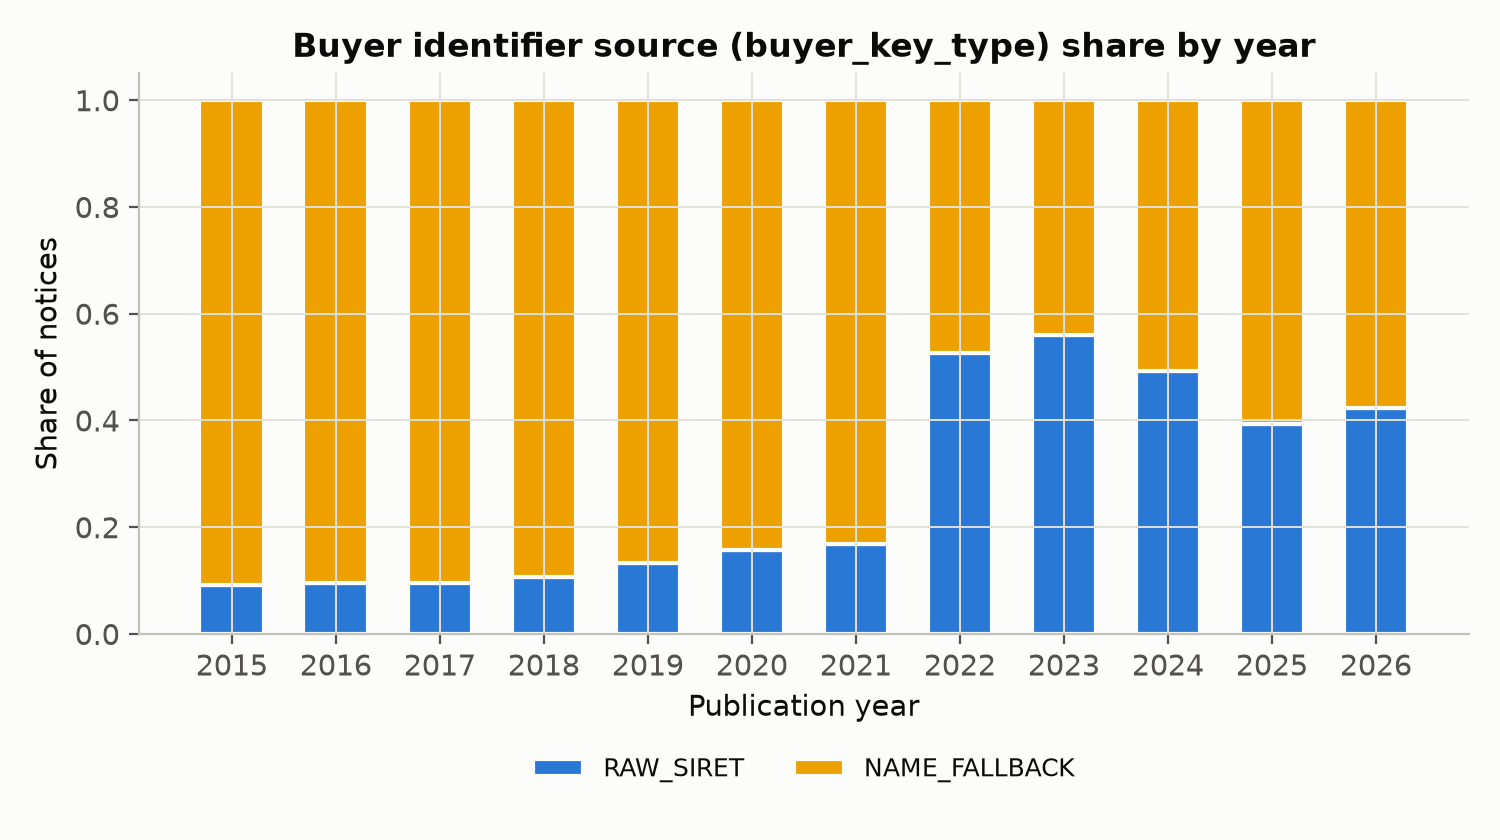
\includegraphics[width=0.85\linewidth]{03_buyer_key_type_by_year.png}
\caption{Buyer-identifier source (\texttt{buyer\_key\_type}) share by
publication year, all 84{,}623 cleaned notices.}
\label{fig:buyerkeytype}
\end{figure}

\begin{figure}[h!]
\centering
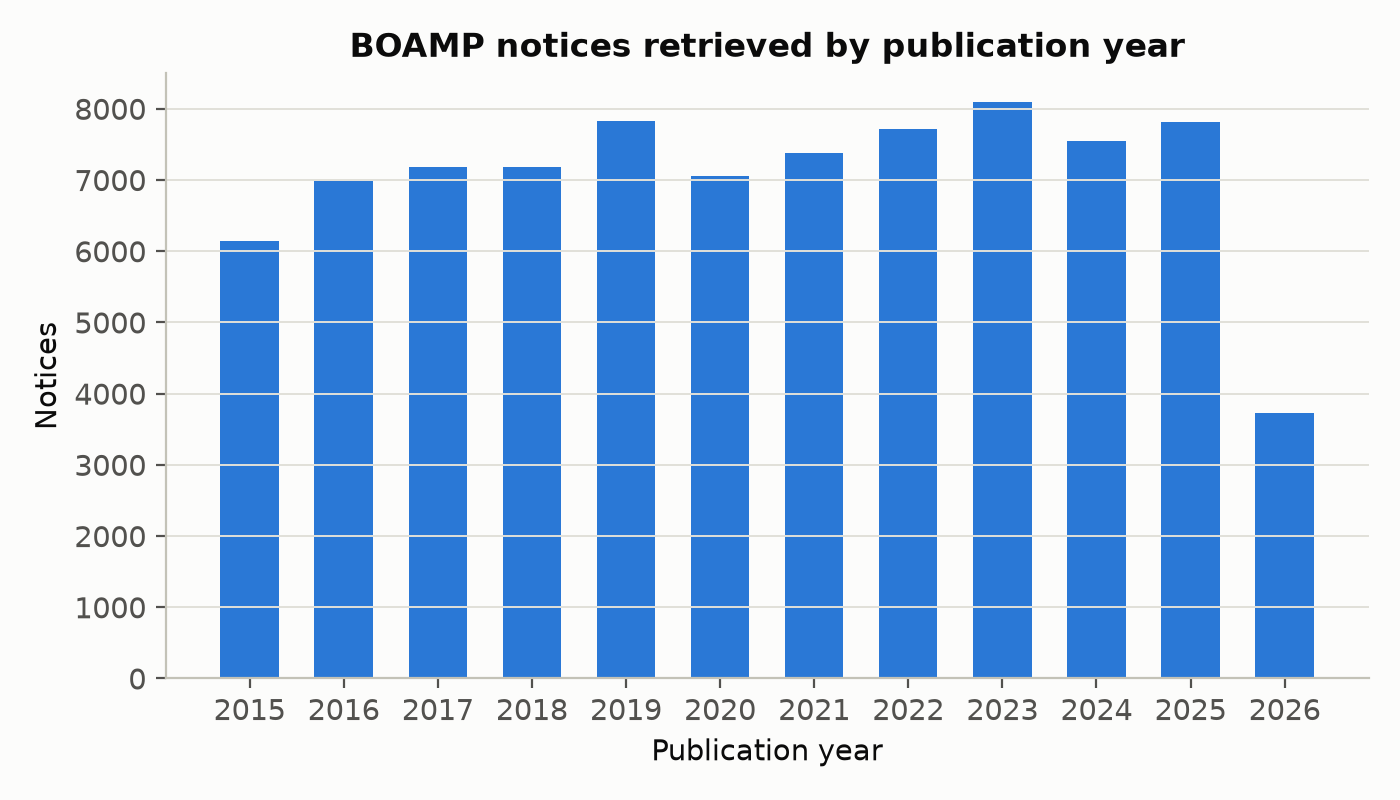
\includegraphics[width=0.48\linewidth]{01_notice_count_by_year.png}
\hfill
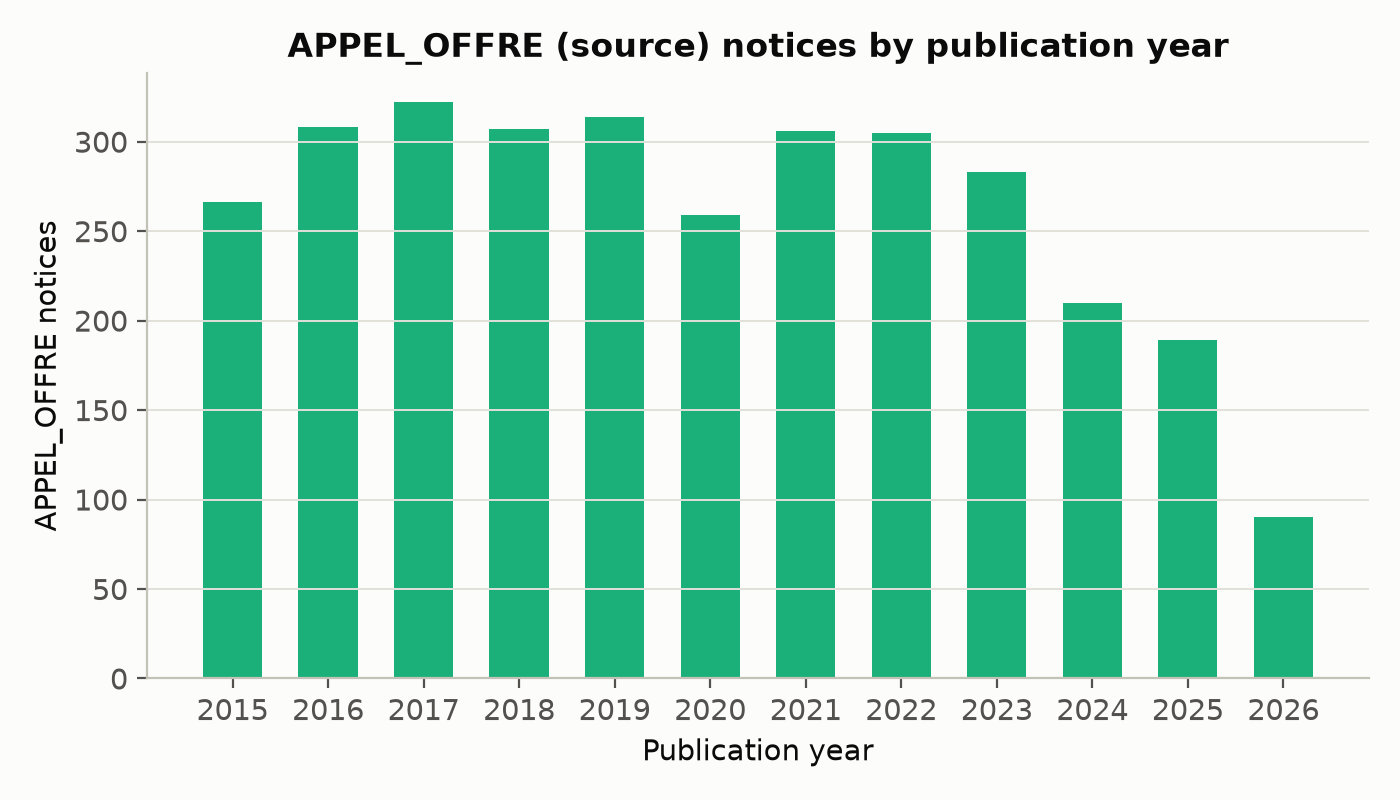
\includegraphics[width=0.48\linewidth]{02_appel_offre_count_by_year.png}
\caption{Left: all cleaned notices by publication year. Right:
\texttt{APPEL\_OFFRE} notices by publication year (all sectors, before the
digital-scope filter).}
\label{fig:noticecounts}
\end{figure}

\section{Dataset Construction and Missing-Value Control}
\label{sec:construction}

\subsection{What Each Dataset Represents}
BOAMP publishes notices, not longitudinal contract histories; a BOAMP row is
one publication event. The pipeline therefore transforms a notice-level
source into a contract-level survival dataset through six persisted stages
(Table~\ref{tab:lineage}).

\begin{table}[h!]
\centering
\caption{Official current data lineage
(\texttt{reports/tables/audit\_data\_lineage.csv},
\texttt{audit\_dataset\_inventory.csv}).}
\label{tab:lineage}
\footnotesize
\begin{tabular}{p{0.30\textwidth}p{0.10\textwidth}rrp{0.22\textwidth}}
\toprule
Dataset & Unit & Rows & Cols & Creation script \\
\midrule
\texttt{boamp\_raw\_flattened.csv} & notice & 84{,}623 & 42 & \texttt{parse\_boamp.py} \\
\texttt{boamp\_clean\_m0\_no\_enrichment.csv} & notice & 84{,}623 & 93 & \texttt{preprocess\_boamp\_m0.py} \\
\texttt{boamp\_m0\_sources.csv} & source notice & 3{,}159 & 22 & \texttt{preprocess\_boamp\_m0.py} \\
\texttt{boamp\_m0\_candidate\_pairs.csv} & source--candidate pair & 6{,}137 & 19 & \texttt{build\_m0\_candidate\_pairs.py} \\
\texttt{boamp\_m0\_links\_balanced.csv} & accepted link & 618 & 21 & \texttt{run\_m0\_linkage.py} \\
\texttt{boamp\_survival\_m0\_balanced.csv} & survival unit & 3{,}159 & 18 & \texttt{run\_m0\_linkage.py} \\
\bottomrule
\end{tabular}
\end{table}

The 84{,}623-row cleaned table describes the available BOAMP evidence across
\emph{all} sectors and notice types; the 3{,}159-row source population
describes possible digital-scope recurrence-source contracts; the
survival handoff is the population on which every result in
Sections~\ref{sec:reliability}--\ref{sec:sensitivity} is measured.

\subsection{How Missing Values Are Handled}
The guiding rule, applied consistently across the pipeline, is
\textbf{flag first, preserve raw values, impute only when a downstream
step truly needs a value}. Table~\ref{tab:missing} documents the main
decisions.

\begin{table}[h!]
\centering
\caption{Main missing-value and quality-control decisions.}
\label{tab:missing}
\small
\begin{tabular}{p{0.16\textwidth}p{0.28\textwidth}p{0.48\textwidth}}
\toprule
Field & Observed quality & Handling rule \\
\midrule
Buyer identity & 27.2\% of all notices carry a format-valid raw SIRET (99.6\% of those also pass checksum). & Use \texttt{SIRET:\ldots} when a valid 14-digit SIRET exists; else \texttt{NAME:\ldots} from a normalized buyer name; \texttt{buyer\_key\_type} records which rule fired. No row is ever dropped for missing buyer identity --- 0\% \texttt{MISSING} across all 84{,}623 notices. \\
CPV code & 78.4\% of M0 sources have a cleaned 8-digit CPV code (down to 45--51\% in 2024--2026, Section~\ref{sec:dq}). & Derive the full hierarchy (\texttt{cpv\_division}/\texttt{group}/\texttt{class}/\texttt{category}); flag division-only ``generic'' codes (9.15\% of sources) separately; a missing CPV in a candidate pair is scored as a distinct \texttt{CPV\_SCORE\_MISSING}=0.1 (Section~\ref{sec:algo}), never as an arbitrary neutral 0.5 and never as evidence of non-match. \\
Contract duration & Only 12.0\% of M0 sources (378 of 3{,}159) have a directly observed, in-range declared duration; 88.0\% required imputation. & Keep the raw declared value when in $[1,120]$ months; else impute the median \emph{observed} duration within the same CPV division (falling back to the global observed median). \texttt{dur\_was\_imputed} records this choice and is itself used as a survival covariate. \\
Contract start date & \texttt{ATTRIBUTION}-linked award dates cover 38.2\% of eligible AO sources (1{,}207/3{,}159). & Use the linked \texttt{ATTRIBUTION} notice's publication date when \texttt{annonce\_lie} resolves it; else fall back to the source's own \texttt{dateparution}. \texttt{start\_date\_source} records which rule fired. \\
Recurrence outcome & BOAMP has no explicit recurrence label. & Build \texttt{event} by the M0 linking rule (Section~\ref{sec:algo}). If no accepted link is found before the study end date, \texttt{event}=0 and the row is right-censored, not deleted. \\
\bottomrule
\end{tabular}
\end{table}

\subsection{Why Right-Censoring Is Not Missing Data}
The reference survival handoff contains 618 linked sources
(\texttt{event}=1) and 2{,}541 unlinked-but-eligible sources
(\texttt{event}=0), for a censoring rate of 80.4\%. The unlinked rows are
\emph{not} removed: they still carry valid information --- the source was
observed, without a detected recurrence, for a known number of months. In
survival-analysis notation:
\begin{itemize}
  \item \texttt{event}=1: the M0 rule found and accepted a later same-buyer
  notice as a plausible recurrence; \texttt{time\_to\_event\_or\_censor\_months}
  is the gap in months between the source and the accepted candidate's
  publication dates.
  \item \texttt{event}=0: no accepted candidate was found (either zero
  candidates passed blocking, or the best candidate's score fell below the
  variant's threshold); \texttt{time\_to\_event\_or\_censor\_months} is the
  gap between the source's publication date and \texttt{study\_end\_date}
  (2026-07-13, the latest observed publication date in the corpus).
\end{itemize}
Removing censored rows would bias the model toward sources that recurred
quickly and would erase long-running or late-window contracts from the risk
set. An internal construction audit
(\texttt{reports/tables/audit\_survival\_construction\_checks.csv}) verified
zero duplicated survival units, zero event rows with a missing linked
candidate, zero censored rows carrying a candidate ID, zero nonpositive
event/censoring times, and zero events recorded after the study end date.

\section{Data Quality Issues Diagnosed}
\label{sec:dq}

\begin{table}[h!]
\centering
\caption{Data quality issues and their impact on linking, per
\texttt{reports/boamp\_m0\_preprocessing\_report.md} \S15 and
\texttt{reports/tables/m0\_preprocessing\_quality\_checks.csv}.}
\small
\begin{tabular}{p{0.03\textwidth}p{0.16\textwidth}p{0.34\textwidth}p{0.35\textwidth}}
\toprule
\# & Issue & Observation & Impact on linking \\
\midrule
1 & Low SIRET coverage & Only 27.2\% of all notices, 22.6\% of M0 sources, carry a raw BOAMP SIRET. & 77.4\% of M0 sources fall back to a normalized-name buyer key. \\
2 & Buyer name-variant fragmentation & Name-fallback buyers are matched only by exact normalized-name equality (no fuzzy matching implemented). & The same real buyer under two spellings splits into two \texttt{buyer\_key} groups, producing structural false negatives that cannot be recovered by tuning the score. \\
3 & CPV coverage declines in recent years & CPV coverage among M0 sources falls from $\sim$92\% (2022--2023) to 45--51\% (2024--2026), timed with the EU eForms/UBL schema transition (late 2023). & Recent-year \texttt{s\_cpv} scores and generic-CPV shares should be read with this drop in mind (Figure~\ref{fig:cpvcov}). \\
4 & Contract duration is sparsely observed & Only 378/3{,}159 (12.0\%) M0 sources have a valid, non-imputed declared duration; median observed value is 6.0 months (n=378). Spot-checked across publication tiers (FNS 12.2\%, JOUE 13.3\%, MAPA 5.6\% observed) --- consistently low, not an eForms-specific artifact. & Drives 88.0\% duration imputation, which in turn sets the temporal blocking window and the estimated-end-date-centered candidate search (Section~\ref{sec:pipeline}). \\
5 & Duration is a right-skewed, keyword-driven signal & Non-imputed durations cluster at 4 (25.9\%), 48 (21.4\%), 6 (11.9\%), and 5 months (9.0\%) rather than the smooth 12/24/36/48-month administrative ceilings a larger sample might show. & Because so few durations are directly observed, this distribution is itself low-confidence (n=378); see the imputation rule in Table~\ref{tab:missing}. \\
6 & Candidate reuse & In the balanced link set, 618 accepted links point to only 443 unique candidate notices; 121 candidates (27.3\%) are reused by more than one source, max.\ multiplicity 6. & Prevents a naive one-to-one ``renewal'' interpretation without manual review (lots, framework agreements, or generic repeat buyers may be defensible many-to-one cases). \\
7 & Blocking excludes most eligible sources & Only 1{,}236 of 3{,}159 eligible sources (39.1\%) have $\geq$1 scored candidate. & No score-based diagnostic can recover a recurrence for the 1{,}923 zero-candidate sources; this is the single largest ceiling on the balanced event rate (Section~\ref{sec:diagnostics}). \\
8 & Duration circularity & Declared/imputed duration defines the estimated end date, which centers both blocking and the temporal score, and duration also remains available as a downstream survival covariate. & A dedicated leakage audit (Section~\ref{sec:leakage}) shows the estimated duration effect on survival hazard is \emph{not} stable to alternative, duration-independent linkage designs. \\
9 & No verified ground truth & BOAMP provides no renewal field. & Precision/recall of the M0 rule are estimated only indirectly (Fellegi--Sunter mixture, Section~\ref{sec:fs}) and remain unverified against manual labels (Section~\ref{sec:manual}). \\
\bottomrule
\end{tabular}
\end{table}

\begin{figure}[h!]
\centering
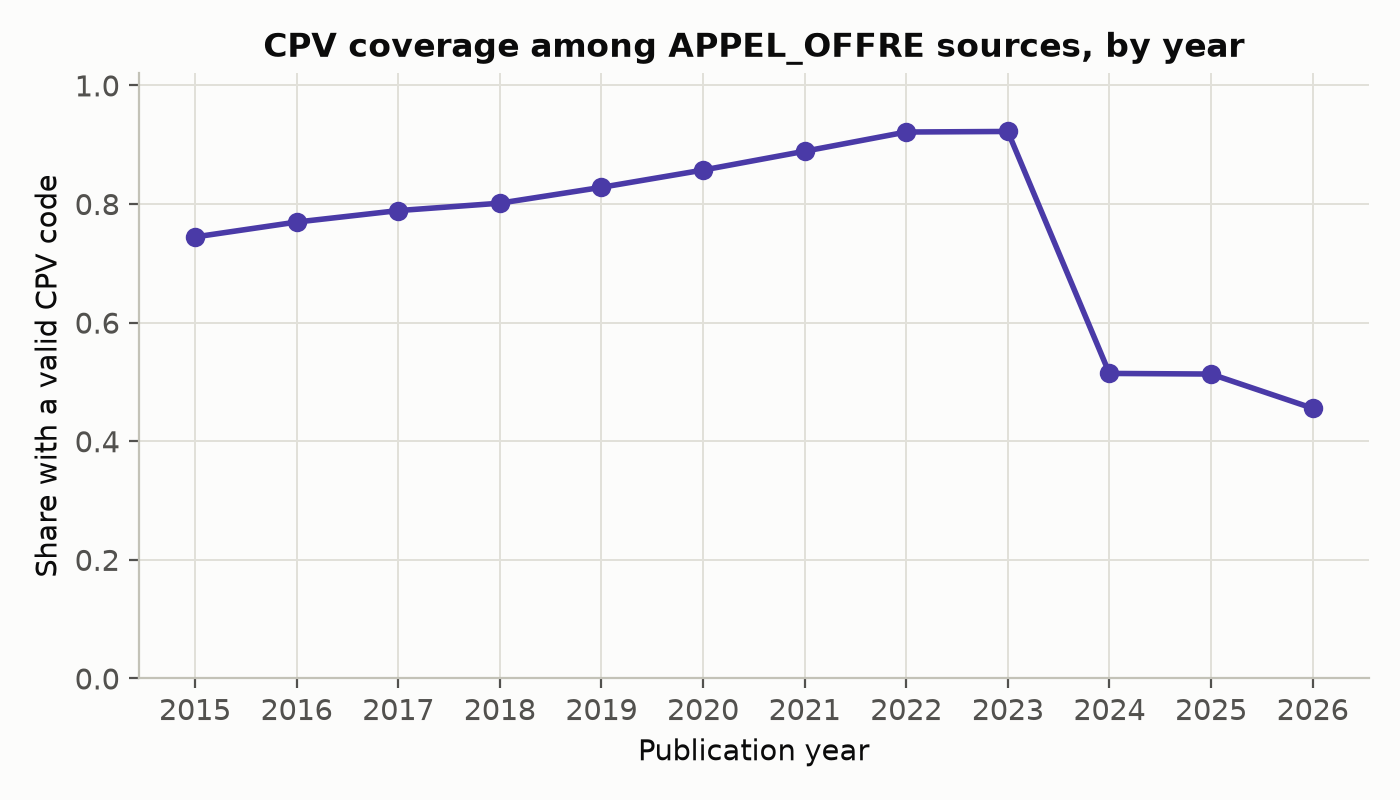
\includegraphics[width=0.48\linewidth]{04_cpv_coverage_by_year.png}
\hfill
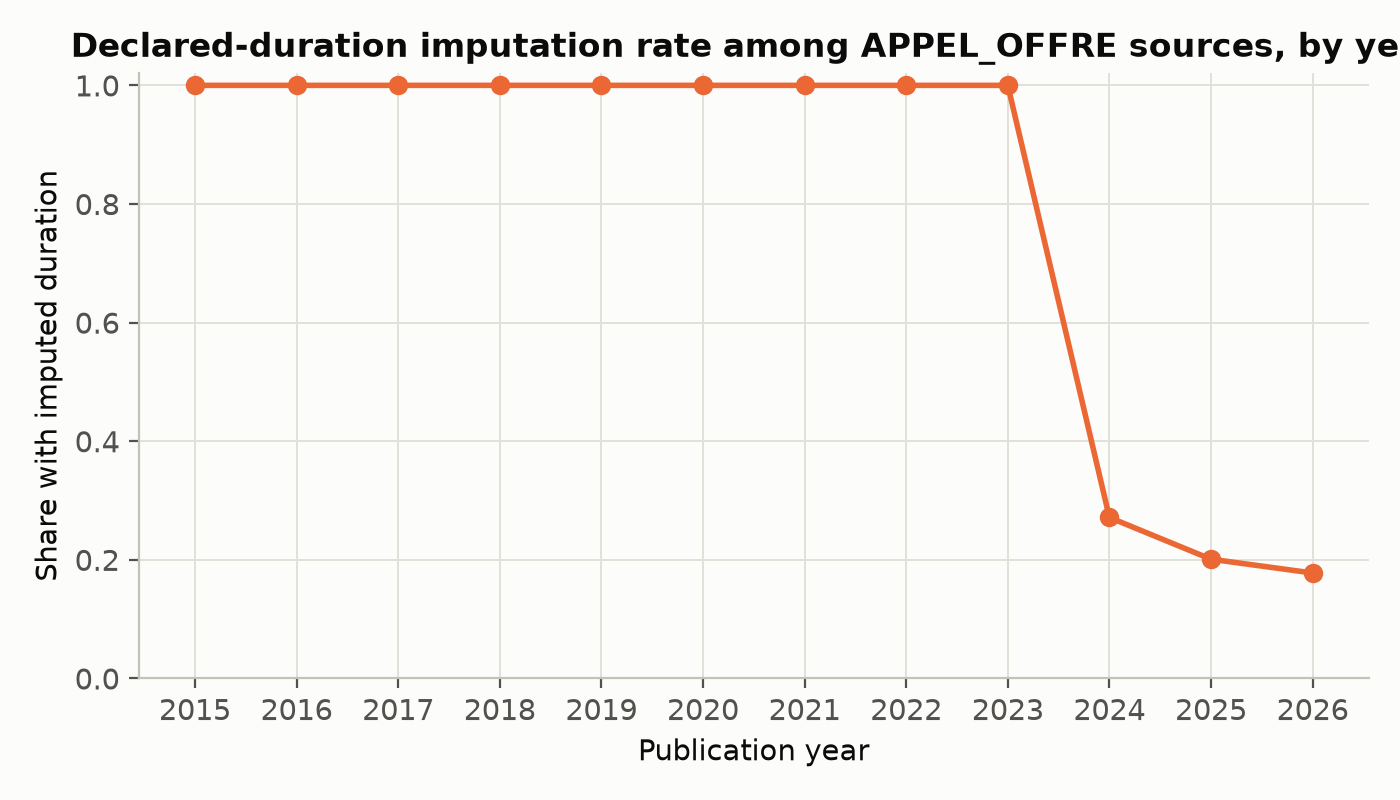
\includegraphics[width=0.48\linewidth]{05_duration_missingness_by_year.png}
\caption{Left: CPV coverage among \texttt{APPEL\_OFFRE} M0 sources, by year
(item 3 above). Right: declared-duration imputation rate among M0 sources,
by year (item 4 above).}
\label{fig:cpvcov}
\end{figure}

\section{Preprocessing Pipeline}
\label{sec:pipeline}

\subsection{Buyer Key Construction}
\label{sec:buyerkey}
For notice $i$ with raw fields $s_i$ (candidate SIRET), $\sigma_i$
(candidate SIREN), and $n_i$ (raw buyer name):
\begin{equation}
\texttt{buyer\_key}_i =
\begin{cases}
\texttt{SIRET:}s_i & \text{if } s_i \text{ passes format \emph{and}\ Luhn checksum validation} \\
\texttt{SIREN:}\sigma_i & \text{else if a valid SIREN is present or derivable from a format-valid SIRET} \\
\texttt{NAME:}\phi(n_i) & \text{else, if } n_i \text{ is present} \\
\texttt{MISSING} & \text{otherwise}
\end{cases}
\end{equation}
where $\phi(\cdot)$ normalizes the buyer name (lowercase, strip accents,
collapse whitespace). This is purely internal cleaning of BOAMP-provided
values, never an external lookup. Across the 3{,}159 M0 sources: 713
(22.6\%) resolve to \texttt{RAW\_SIRET}, 0 to \texttt{RAW\_SIREN} (no
BOAMP notice in this scope carries a raw SIREN without also carrying a
recoverable SIRET), 2{,}446 (77.4\%) to \texttt{NAME\_FALLBACK}, and 0 to
\texttt{MISSING}.

\subsection{Contract Start-Date Refinement}
\begin{equation}
\texttt{start\_date}_i =
\begin{cases}
\texttt{publication\_date}(j) & \text{if } \exists\, j \in \texttt{ATTRIBUTION} : \texttt{annonce\_lie}(j) \ni i,\ \text{earliest such } j \\
\texttt{publication\_date}_i & \text{otherwise}
\end{cases}
\end{equation}
In practice, 1{,}207 of 3{,}159 M0 sources (38.2\%) obtain a more precise
start date via a linked \texttt{ATTRIBUTION} notice; the remaining 61.8\%
fall back to their own publication date.

\subsection{Duration Imputation}
\begin{equation}
d_i =
\begin{cases}
\texttt{declared\_duration\_months}_i & \text{if observed and} \in [1,120]\text{ months} \\
\mathrm{median}\{d_k : k \in \texttt{cpv\_division}(i),\ \text{observed}\} & \text{else, if that median exists} \\
\mathrm{median}\{d_k : \text{observed}, k \in \text{digital-scope AO}\} & \text{else (global fallback)}
\end{cases}
\end{equation}
Medians are computed on the \emph{digital-scope, Pays-de-la-Loire
\texttt{APPEL\_OFFRE}} population only (i.e.\ the 3{,}159-row M0 source
population), so imputed durations reflect in-scope contracts rather than
importing behavior from other sectors. 2{,}781 of 3{,}159 sources (88.0\%)
receive an imputed value (\texttt{dur\_was\_imputed}=\texttt{True}).

\subsection{Estimated End Date}
\begin{equation}
\hat e_i = \texttt{start\_date}_i + d_i \text{ months}
\end{equation}
This is the center of both the temporal-blocking window
(Section~\ref{sec:algo}) and the survival-relevant ``expected recurrence
date.''

\subsection{CPV Cleaning and Hierarchy}
A raw CPV code is kept only if it matches an 8-digit pattern; from it,
\texttt{cpv\_division} (2 digits), \texttt{cpv\_group} (3), \texttt{cpv\_class}
(4), and \texttt{cpv\_category} (5) are derived by left truncation. A code
ending in six zeros (\texttt{XX000000}) is flagged \texttt{cpv\_generic\_flag}
= \texttt{True}, since it carries no sub-division signal.

\subsection{Text Normalization}
The free-text \texttt{objet} field is cleaned (\texttt{clean\_objet}: strip
boilerplate, normalize whitespace/accents) into \texttt{objet\_clean}, which
feeds a TF-IDF vectorizer (\texttt{scikit-learn}, unigrams+bigrams,
\texttt{max\_features=50{,}000}, \texttt{min\_df=2}) fitted over all 3{,}159
eligible source texts. Sentence-Transformer embeddings were evaluated for
this step but not adopted: at the pipeline's original national scale
($\sim$340k notices) CPU-only transformer embedding was judged impractical,
and TF-IDF+cosine was kept for continuity even though the current
Pays-de-la-Loire/digital scope (3{,}159 sources) is small enough that
embeddings would now be tractable --- listed as a next step in
\texttt{reports/boamp\_m0\_preprocessing\_report.md} \S16.

\section{Recurrence-Linking Algorithm (M0)}
\label{sec:algo}

\subsection{Position in the Record-Linkage Literature}
Methodologically, M0 is a \emph{record-linkage} problem in the classical
sense of Fellegi and Sunter \cite{fellegi1969}: deciding, from a vector of
field-comparison scores, whether two records refer to the same underlying
entity --- here, the same recurring procurement need rather than the same
person or firm. The two standard ingredients both appear in M0 in
deterministic form: \emph{blocking} (restricting comparisons to pairs
sharing a cheap, high-precision key --- here the buyer key plus a temporal
window \cite{christen2012}) and \emph{comparison-vector scoring} (here a
fixed linear combination rather than estimated log-likelihood ratios).
What is project-specific is (i) the target relation itself --- recurrence
of a need, which has no ground-truth registry to link against, unlike
classical deduplication --- and (ii) the deterministic, fully documented
weights, chosen for auditability over statistical optimality. The
probabilistic Fellegi--Sunter machinery is used in this project only
\emph{diagnostically}, as an unsupervised mixture re-analysis of M0's
comparison vectors (Section~\ref{sec:fs}), not as the linkage rule.

\subsection{Notation}
Let $i$ index an eligible source notice (non-\texttt{MISSING} buyer key)
and $j$ a later candidate notice from the \emph{same} buyer key. Each
notice carries a publication date $t$, an estimated end date $\hat e$ (for
sources), a CPV hierarchy, cleaned object text, and a buyer-key type.

\subsection{Step 1 --- Eligibility and Candidate Pool}
The temporal window is derived from data, not hardcoded:
\begin{equation}
W = \mathrm{clip}\big(\mathrm{round}(0.5 \times \tilde d_{\text{obs}}),\ 6,\ 24\big) \text{ months}
\end{equation}
where $\tilde d_{\text{obs}}=6.0$ months is the median \emph{observed}
(non-imputed) duration among M0 sources (Section~\ref{sec:dq}, item~4).
This gives $W = \mathrm{clip}(3, 6, 24) = 6$ months. The realized candidate
universe is
\begin{equation}
\Omega = \big\{(i,j) : \texttt{buyer\_key}(j)=\texttt{buyer\_key}(i),\ t_j > t_i,\ |t_j - \hat e_i| \leq W \big\},
\end{equation}
capped, per source, at the 30 temporally nearest candidates
(\texttt{MAX\_CANDIDATES\_PER\_SOURCE}) for runtime; this cap did not bind
in the current (much smaller than the pipeline's original national) scope.
$\Omega$ contains 6{,}137 pairs covering 1{,}236 of the 3{,}159 eligible
sources (39.1\% blocking coverage, Section~\ref{sec:diagnostics}).

\subsection{Step 2 --- Component Scores}
\textbf{Text similarity} is TF-IDF \cite{salton1988} cosine similarity
between source and candidate object text:
\begin{equation}
s_{\text{text}}(i,j) = \frac{\mathbf v_i \cdot \mathbf v_j}{\lVert \mathbf v_i\rVert \lVert \mathbf v_j\rVert} \in [0,1].
\end{equation}

\textbf{CPV compatibility} follows the official CPV hierarchy (division /
group / class / category / full 8-digit code), rewarding the depth of the
longest shared prefix:
\begin{equation}
s_{\text{cpv}}(i,j) =
\begin{cases}
0.1 & \text{either CPV missing} \\
1.0 & \text{identical full 8-digit code} \\
0.8 & \text{same 5-digit category} \\
0.6 & \text{same 4-digit class} \\
0.4 & \text{same 3-digit group} \\
0.2 & \text{same 2-digit division} \\
0.0 & \text{valid CPVs, different divisions}
\end{cases}
\end{equation}
A missing CPV is scored 0.1 --- a documented weak-neutral value, distinct
from and strictly lower than any confirmed match, but not treated as
evidence \emph{against} the pair the way a confirmed cross-division
mismatch (0.0) is.

\textbf{Temporal proximity} decays linearly from 1.0 at the estimated end
date to 0.0 at the window boundary:
\begin{equation}
s_{\text{time}}(i,j) = \mathrm{clip}\!\left(1 - \frac{|(t_j-t_i) - d_i|}{W},\ 0,\ 1\right).
\end{equation}

\textbf{Buyer-key reliability} reflects how trustworthy the
already-enforced buyer-key match is, not whether it matched (candidate
generation already conditions on identical \texttt{buyer\_key}):
\begin{equation}
s_{\text{buyer}}(i) =
\begin{cases}
1.00 & \texttt{buyer\_key\_type} = \texttt{RAW\_SIRET} \\
0.85 & \texttt{buyer\_key\_type} = \texttt{RAW\_SIREN} \\
0.60 & \texttt{buyer\_key\_type} = \texttt{NAME\_FALLBACK}
\end{cases}
\end{equation}

\subsection{Step 3 --- Composite Score}
\begin{equation}
S(i,j) = 0.35\, s_{\text{text}} + 0.30\, s_{\text{cpv}} + 0.25\, s_{\text{time}} + 0.10\, s_{\text{buyer}} \in [0,1].
\end{equation}
Weights are documented, fixed choices, not fitted: text and CPV are treated
as the primary content-based recurrence signals, timing anchors the match
around the expected end date, and the buyer-reliability term mostly
discounts low-confidence name-only matches without changing the ranking
\emph{within} a source's candidate pool (since it is constant across all of
that source's candidates). Weights were reviewed against the observed score
distribution (mean composite score 0.250 over all pairs) but not re-tuned
against a validation set, to avoid overfitting to a single run's
distribution.

\subsection{Step 4 --- Best-Match Selection and Threshold Variants}
For each source with $\geq 1$ candidate, candidates are ranked by $S(i,j)$
and the rank-1 (best) candidate's score is kept. Three link \emph{variants}
are derived from the 25th/50th/75th percentile of the rank-1 score
distribution ($n=1{,}236$), not from an a-priori cutoff:

\begin{table}[h!]
\centering
\caption{M0 link variants (\texttt{reports/tables/m0\_method\_summary.csv}).
Denominator is the full eligible population, 3{,}159 sources.}
\label{tab:variants}
\small
\begin{tabular}{lrrrr}
\toprule
Variant & Threshold $\tau$ & Linked events & Event rate & Median gap \\
\midrule
Broad & 0.2642 (p25) & 927 & 29.3\% & 37.9 months \\
\textbf{Balanced (reference)} & \textbf{0.3230 (p50)} & \textbf{618} & \textbf{19.6\%} & \textbf{37.7 months} \\
Strict & 0.3931 (p75) & 309 & 9.8\% & 44.7 months \\
\bottomrule
\end{tabular}
\end{table}
Because all three thresholds are cuts on the \emph{same} rank-1 score
distribution, the sets are nested: \texttt{strict} $\subset$
\texttt{balanced} $\subset$ \texttt{broad}. The reference outcome variable
is
\begin{equation}
\texttt{event}_i =
\begin{cases}
1 & \text{if } \exists j : S(i,j) = \max_k S(i,k) \geq \tau_{\text{balanced}} \\
0 & \text{otherwise}
\end{cases}
\end{equation}
\texttt{event}=0 means \emph{no accepted candidate under the current rule},
not verified evidence that no recurrence occurred.

\begin{figure}[h!]
\centering
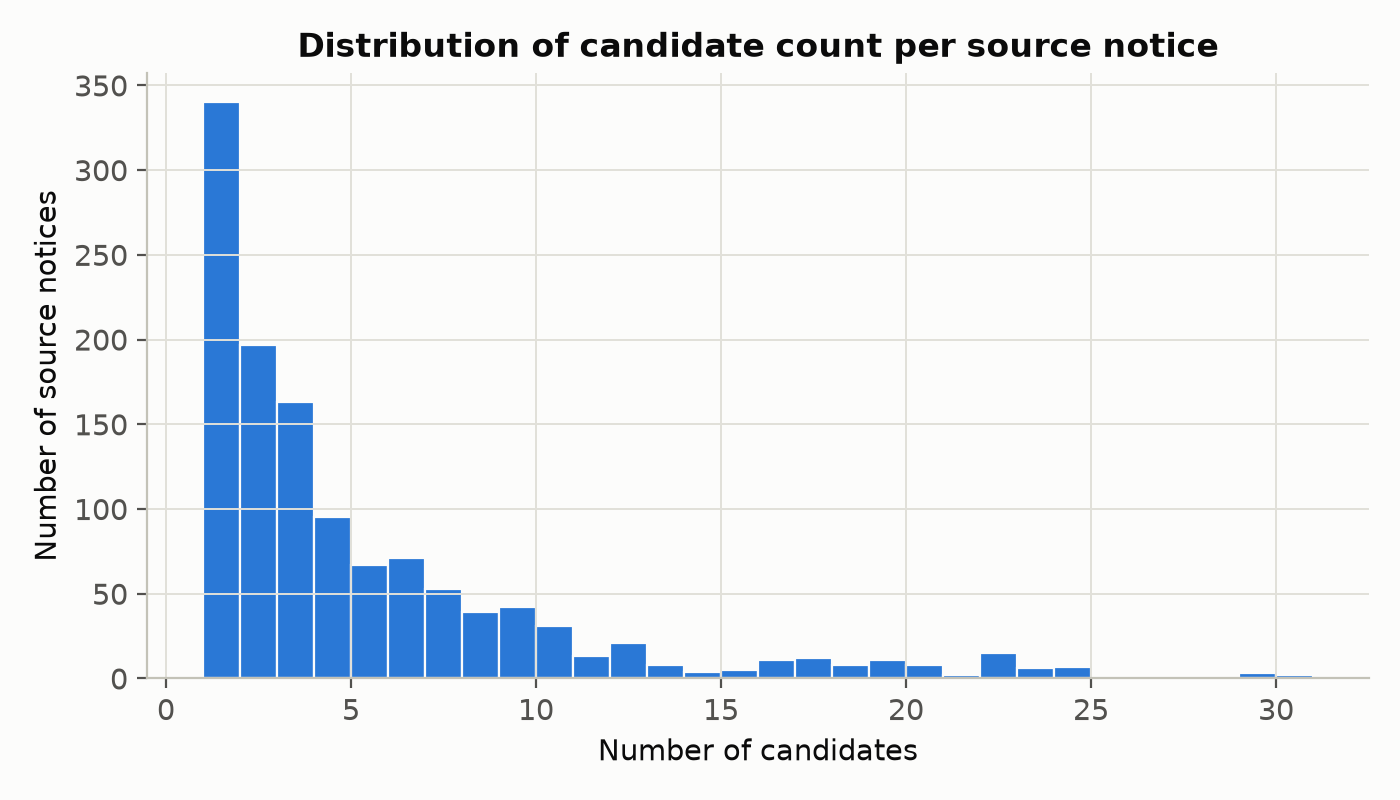
\includegraphics[width=0.48\linewidth]{06_candidate_count_distribution.png}
\hfill
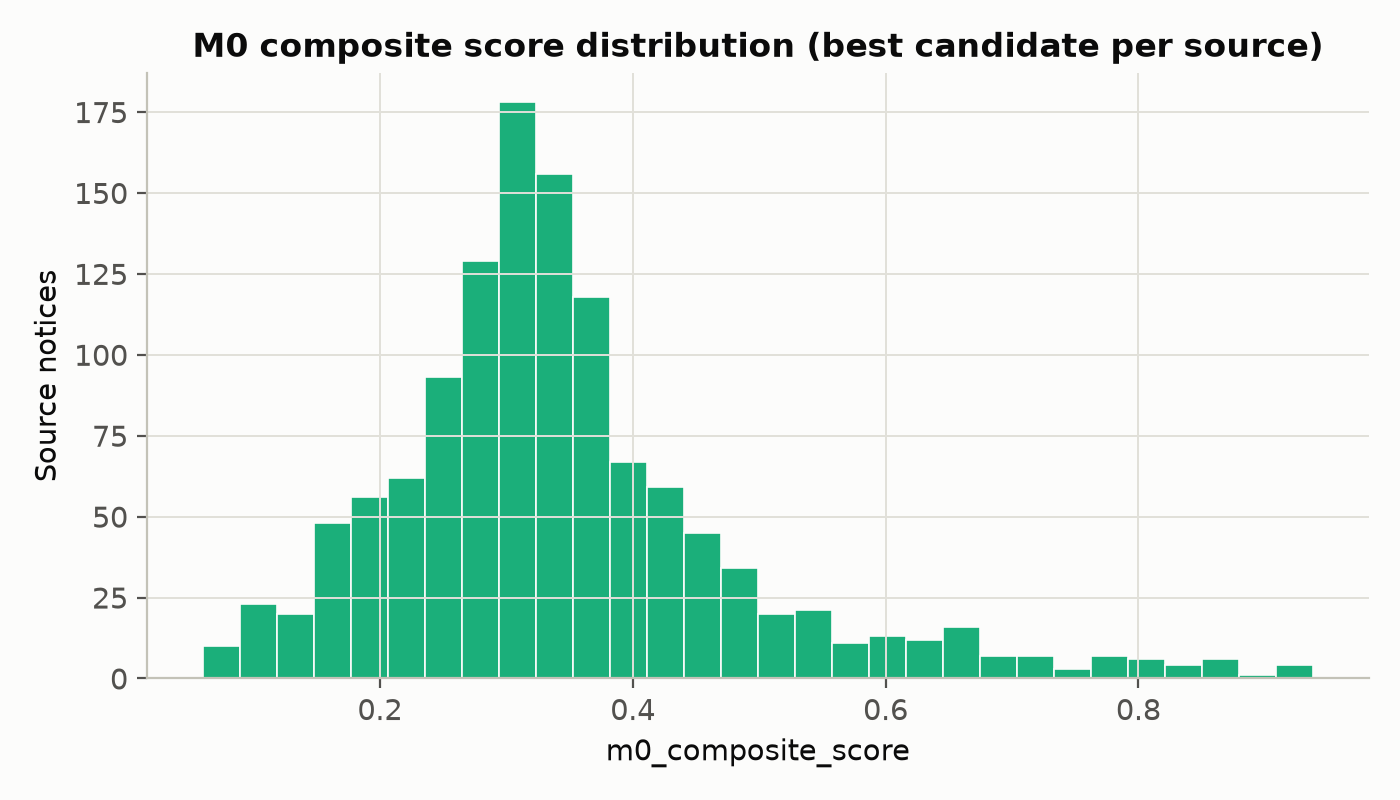
\includegraphics[width=0.48\linewidth]{07_m0_score_distribution.png}
\caption{Left: distribution of the number of scored candidates per source
notice, among the 1{,}236 sources with $\geq 1$ candidate. Right:
distribution of the best (rank-1) composite score per source, with the
broad/balanced/strict thresholds marked.}
\label{fig:candidatescore}
\end{figure}

\section{Output Dataset --- Survival Handoff}
\label{sec:output}

\subsection{File: \texttt{boamp\_survival\_m0\_balanced.csv}}
One row per eligible source notice (3{,}159 rows, 18 columns); the official
Phase-2 modeling input.

\begin{table}[h!]
\centering
\caption{Column dictionary --- \texttt{boamp\_survival\_m0\_balanced.csv}.}
\small
\begin{tabular}{p{0.28\textwidth}p{0.08\textwidth}p{0.55\textwidth}}
\toprule
Column & Type & Description \\
\midrule
\texttt{notice\_id} & string & Source \texttt{APPEL\_OFFRE} BOAMP ID. \\
\texttt{buyer\_key} / \texttt{buyer\_key\_type} & string & Grouping key and its provenance (RAW\_SIRET / NAME\_FALLBACK). \\
\texttt{publication\_date}, \texttt{start\_date}, \texttt{estimated\_end\_date}, \texttt{study\_end\_date} & date & Temporal anchors (Section~\ref{sec:pipeline}). \\
\texttt{cpv\_division}, \texttt{cpv\_category}, \texttt{category\_label} & string & Classification of the source contract; \texttt{category\_label} is binary (\texttt{DIGITAL\_ICT} for every row here, since the file is already scope-filtered). \\
\texttt{declared\_duration\_months} & float & Observed or imputed duration (Section~\ref{sec:pipeline}). \\
\texttt{dur\_was\_imputed} & bool & True for 2{,}781/3{,}159 rows (88.0\%). \\
\texttt{event} & int & \textbf{Target variable}. 1 = accepted M0 link (618 rows), 0 = no accepted link (2{,}541 rows). \\
\texttt{time\_to\_event\_or\_censor\_months} & float & Survival time, always filled. For \texttt{event}=1: gap in months between source and linked candidate publication dates. For \texttt{event}=0: gap between source publication date and \texttt{study\_end\_date}. \\
\texttt{linked\_candidate\_notice\_id} & string & Accepted candidate's BOAMP ID; empty when \texttt{event}=0. \\
\texttt{m0\_composite\_score} & float & $S(i,j^*)$ for linked rows; empty when \texttt{event}=0. \\
\texttt{variant} & string & Constant \texttt{"balanced"} in this file. \\
\bottomrule
\end{tabular}
\end{table}

\subsection{Score Distributions for Linked Events}
Table~\ref{tab:scorepop} compares component-score statistics across five
populations: all 6{,}137 candidate pairs, the 1{,}236 rank-1 (best)
candidates, the 618 accepted balanced links, the 5{,}519 rejected
candidates, and the 896 runner-up candidates (rank-2 among sources with
$\geq 2$ candidates). This is a placebo-style comparison: if the composite
score carried no discriminative signal, accepted links and runner-ups would
have similar distributions.

\begin{table}[h!]
\centering
\caption{Composite score by population (source:
\texttt{reports/tables/}\newline\texttt{audit\_score\_component\_distributions.csv}).}
\label{tab:scorepop}
\small
\begin{tabular}{lrrrr}
\toprule
Population & $n$ & Mean $S$ & Median $S$ & Mean margin $m$ \\
\midrule
All candidate pairs & 6{,}137 & 0.250 & 0.241 & 0.086 \\
Rank-1 (best) candidates & 1{,}236 & 0.345 & 0.323 & 0.137 \\
\textbf{Accepted balanced links} & \textbf{618} & \textbf{0.444} & \textbf{0.393} & \textbf{0.161} \\
Rejected candidates & 5{,}519 & 0.229 & 0.226 & 0.077 \\
Runner-up candidates & 896 & 0.287 & 0.289 & 0.080 \\
\bottomrule
\end{tabular}
\end{table}
The mean composite score of accepted links (0.444) is well above the
rejected-candidate mean (0.229), and the margin $m$ (best minus second-best
score) is also larger for accepted links (0.161) than for the ambient
candidate pool (0.086), consistent with the score being internally
discriminative (Section~\ref{sec:margin} quantifies this further).

\section{Linking Diagnostics}
\label{sec:diagnostics}

\subsection{Blocking Coverage}
\label{sec:blocking}
Of 3{,}159 eligible sources, only 1{,}236 (39.1\%) have $\geq 1$ scored
candidate; 1{,}923 (60.9\%) have zero. No downstream score-based diagnostic
--- Fellegi--Sunter posteriors, threshold sensitivity, corruption recovery
--- can recover a recurrence signal for these 1{,}923 sources, since they
never enter $\Omega$. Coverage decays sharply toward the end of the study
period (Table~\ref{tab:blockyear}), the expected signature of finite
follow-up combined with duration-centered blocking.

\begin{table}[h!]
\centering
\caption{Blocking coverage by publication year
(\texttt{reports/tables/audit\_blocking\_coverage.csv}).}
\label{tab:blockyear}
\begin{tabular}{rrrrr}
\toprule
Year & Eligible sources & With candidate & Zero candidate & Coverage \\
\midrule
2015 & 266 & 151 & 115 & 56.8\% \\
2016 & 308 & 177 & 131 & 57.5\% \\
2017 & 322 & 191 & 131 & 59.3\% \\
2018 & 307 & 156 & 151 & 50.8\% \\
2019 & 314 & 165 & 149 & 52.5\% \\
2020 & 259 & 109 & 150 & 42.1\% \\
2021 & 306 & 95 & 211 & 31.0\% \\
2022 & 305 & 60 & 245 & 19.7\% \\
2023 & 283 & 18 & 265 & 6.4\% \\
2024 & 210 & 50 & 160 & 23.8\% \\
2025 & 189 & 53 & 136 & 28.0\% \\
2026 (partial) & 90 & 11 & 79 & 12.2\% \\
\bottomrule
\end{tabular}
\end{table}
Coverage also varies by buyer publication frequency: 0\% for buyers with a
single digital AO notice in the whole period (386 sources, structurally
excluded), rising to 69.0\% for buyers with 26+ digital AO notices (963
sources). \texttt{RAW\_SIRET}-keyed sources have \emph{lower} coverage
(29.3\%) than \texttt{NAME\_FALLBACK}-keyed sources (42.0\%) --- a
reminder that buyer-key reliability and blocking coverage are not the same
axis of credibility.

\subsection{Zero-Candidate Failure Analysis}
The audit table \texttt{audit\_censoring\_diagnostics.csv} decomposes the
1{,}923 zero-candidate sources into two structurally distinct causes,
distinguished from the 1{,}236 sources that \emph{do} have candidates:

\begin{table}[h!]
\centering
\caption{Zero-candidate failure decomposition (all 3{,}159 eligible sources).}
\begin{tabular}{p{0.32\textwidth}rp{0.44\textwidth}}
\toprule
Cause & Count & Interpretation \\
\midrule
Has $\geq 1$ candidate & 1{,}236 & Enters $\Omega$; may or may not clear the balanced threshold. \\
No later same-buyer notice at all & 798 & Structural: this buyer published no further digital AO in the study period. \\
Later notices exist, but all fall outside the $\pm 6$-month window & 1{,}125 & Structural: recurrence timing (if any) is outside the duration-implied search window. \\
\bottomrule
\end{tabular}
\end{table}
The temporal-window-excluded cause (1{,}125 sources, 35.6\% of all
eligible sources) is the largest single failure mode and is directly tied
to the duration-centered blocking design audited in
Section~\ref{sec:leakage}; Section~\ref{sec:worked} gives a concrete worked
example of this failure mode.

\subsection{Score Margin and Threshold Sensitivity}
\label{sec:margin}
The score margin $m$ (best minus second-best composite score) is defined
for all 1{,}236 rank-1 candidates: the rank-1-minus-rank-2 score when a
source has $\geq 2$ candidates, or the rank-1 score itself when only one
candidate exists. The mean margin among accepted balanced links is 0.161
(Table~\ref{tab:scorepop}), versus 0.086 across all pairs.

Perturbing the balanced threshold by $\pm\delta$ changes how many rank-1
sources flip event status:

\begin{table}[h!]
\centering
\caption{Threshold perturbation sensitivity
(\texttt{reports/tables/m6a\_threshold\_sensitivity.csv}), around
$\tau_{\text{balanced}}=0.3230$.}
\begin{tabular}{rrr}
\toprule
$\pm\delta$ & Sources flipped & Share of 1{,}236 rank-1 sources \\
\midrule
0.005 & 48 & 3.9\% \\
0.010 & 88 & 7.1\% \\
0.020 & 227 & 18.4\% \\
0.050 & 516 & 41.7\% \\
\bottomrule
\end{tabular}
\end{table}
The balanced threshold sits in a non-negligible mass of the rank-1 score
distribution: borderline cases are common (Figure~\ref{fig:threshsens}) and
should not be presented as individually reliable without manual or external
corroboration.

\begin{figure}[h!]
\centering
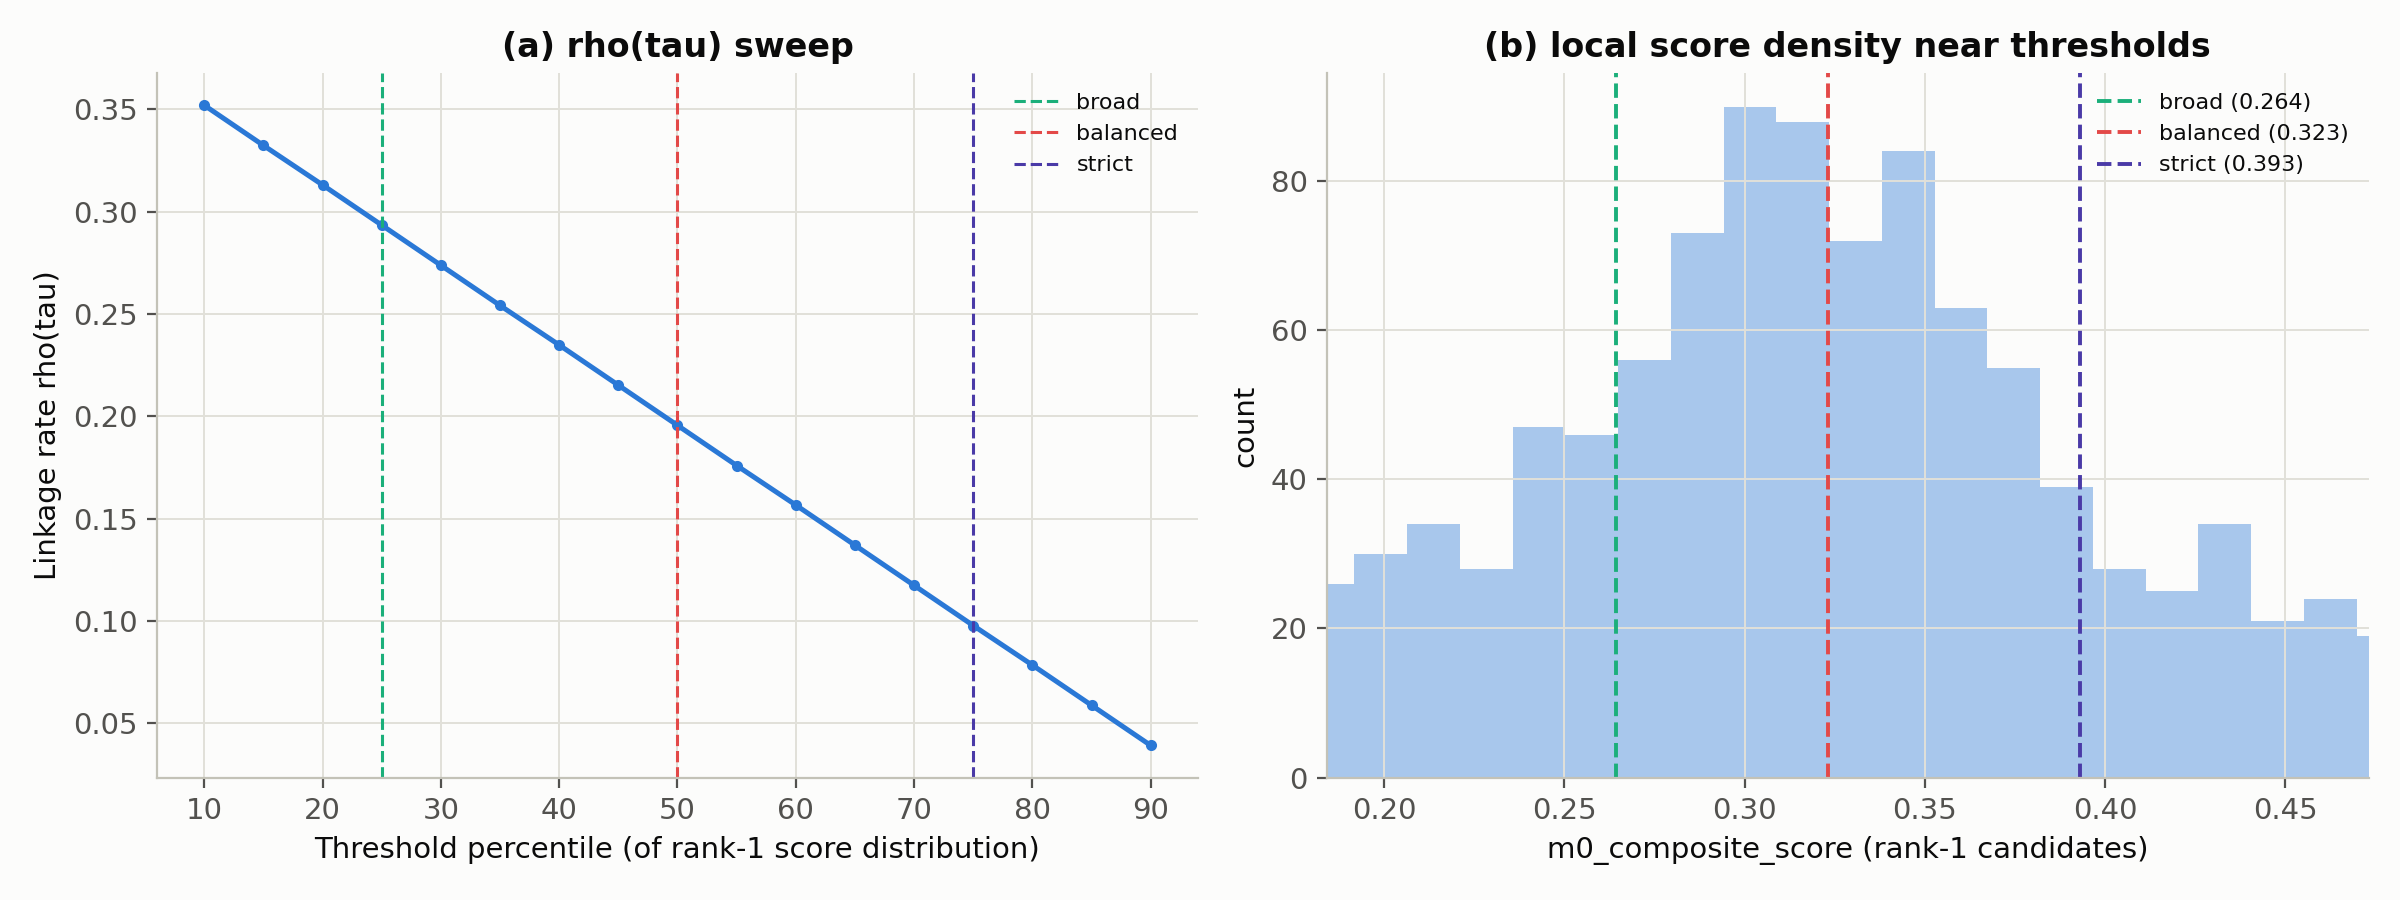
\includegraphics[width=\linewidth]{14_threshold_sensitivity.png}
\caption{(a) Linkage rate $\rho(\tau)$ as the threshold percentile sweeps
from p10 to p90 of the rank-1 score distribution. (b) Local density of
rank-1 scores near the three named thresholds.}
\label{fig:threshsens}
\end{figure}

\subsection{Feature Ablation}
Dropping one score component, renormalizing the remaining weights,
reranking candidates, and rebuilding a same-sized link set gives the
Jaccard overlap with the reference balanced set shown in
Figure~\ref{fig:ablation}. The buyer component is least influential
(Jaccard 0.904) because $s_{\text{buyer}}$ is constant across all
candidates for a given source --- it can move a source above or below
threshold but cannot change which candidate ranks first \emph{within} that
source. Time (Jaccard 0.668) and text (0.684) are the most influential
despite text's larger nominal weight, because both vary continuously
within a candidate pool while CPV is coarser (only 6 discrete rungs).

\begin{figure}[h!]
\centering
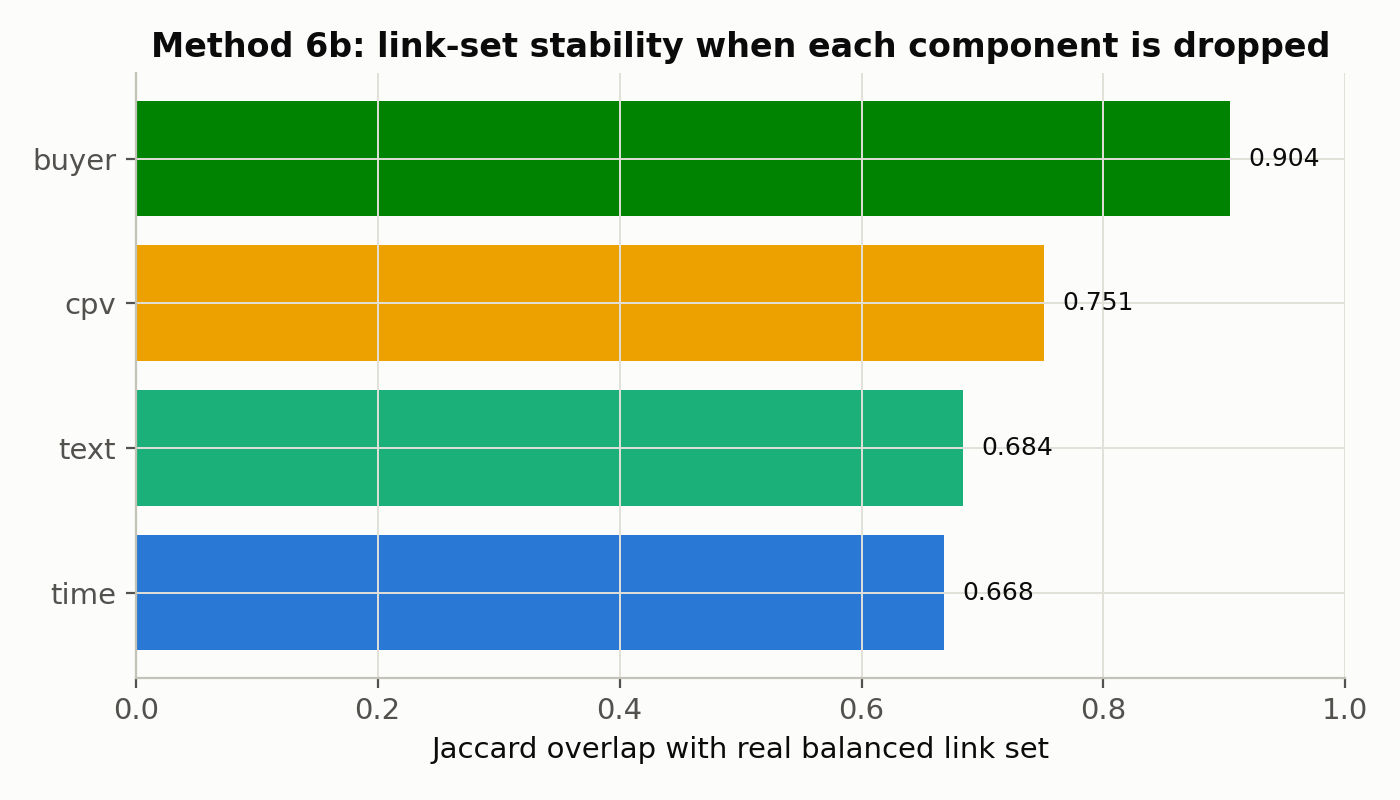
\includegraphics[width=0.75\linewidth]{15_feature_ablation_jaccard.png}
\caption{Link-set stability (Jaccard overlap with the reference balanced
set) when each score component is dropped and weights renormalized.}
\label{fig:ablation}
\end{figure}

\subsection{Linkage Rate by Publication Year}
\begin{figure}[h!]
\centering
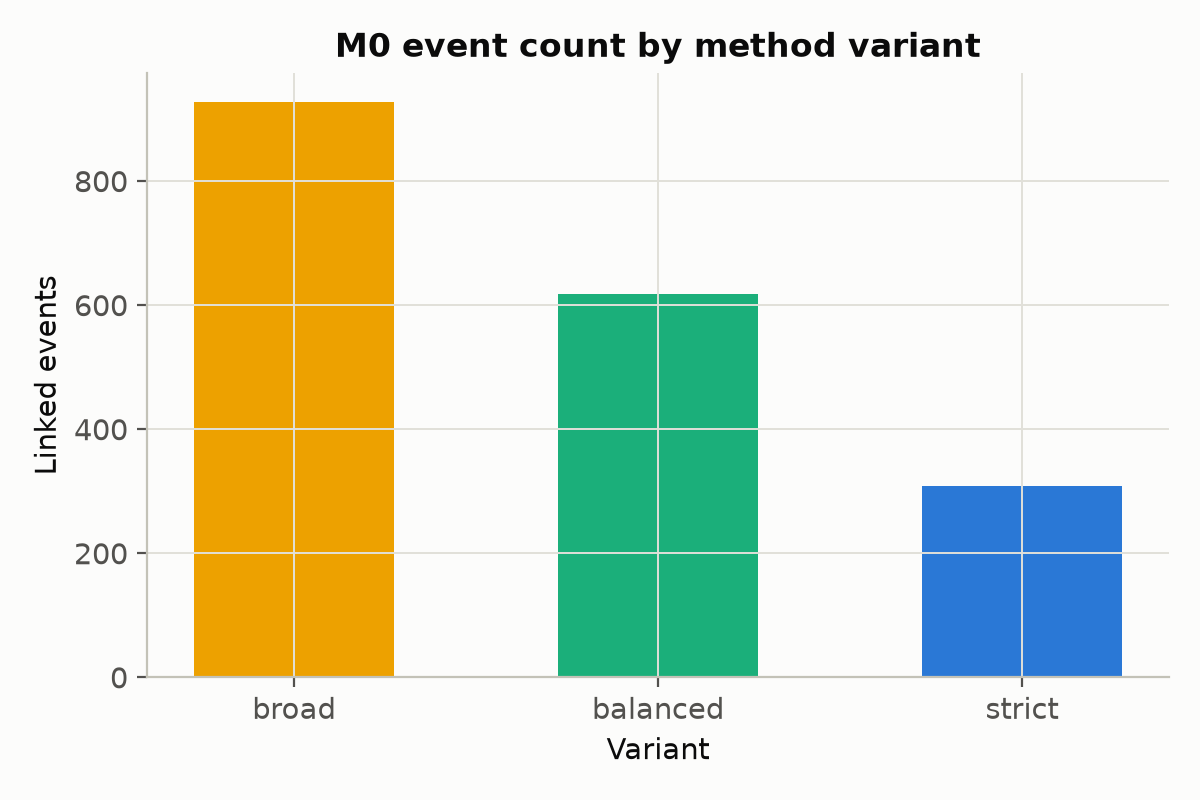
\includegraphics[width=0.48\linewidth]{08_event_count_by_variant.png}
\hfill
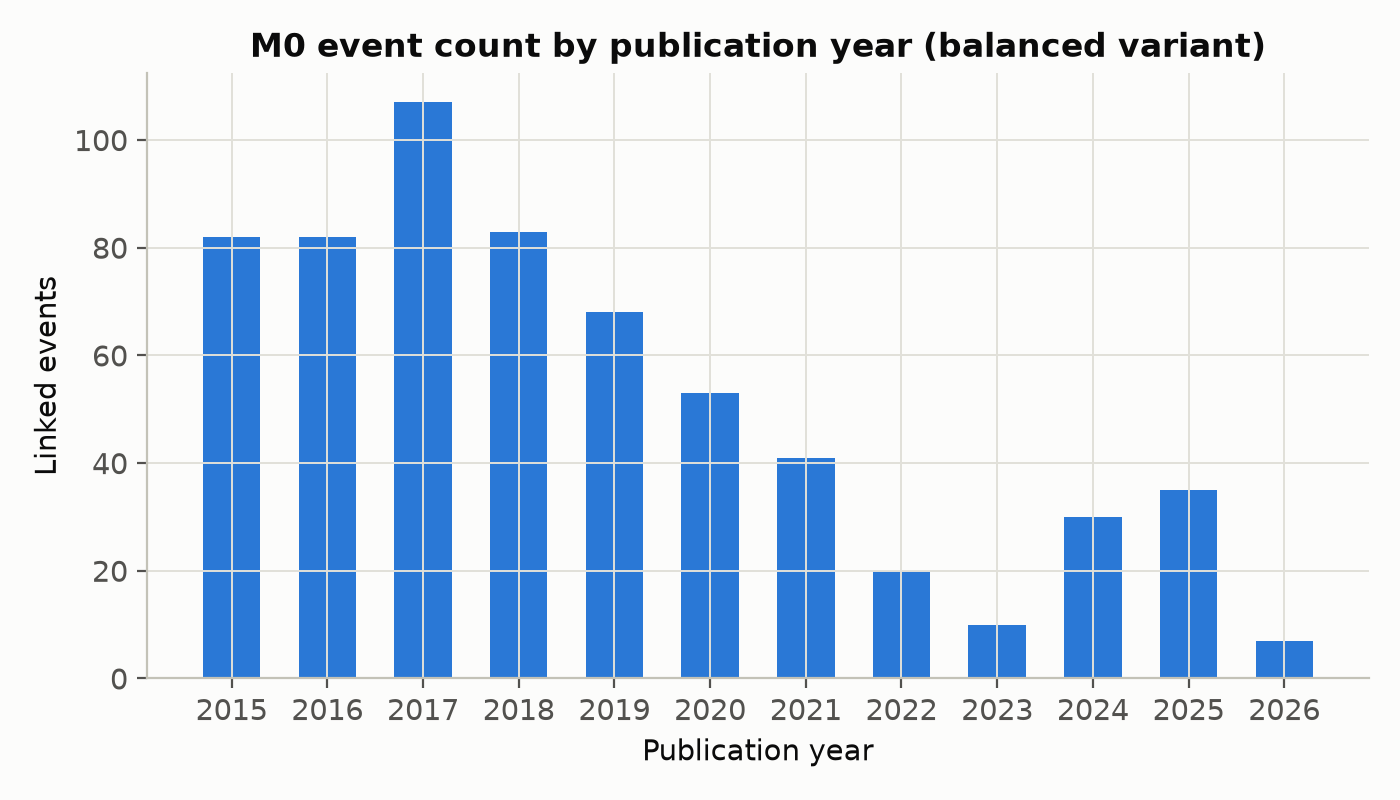
\includegraphics[width=0.48\linewidth]{09_event_count_by_year_balanced.png}
\caption{Left: event count by variant (broad/balanced/strict). Right:
balanced-variant event count by publication year --- coverage decay
(Table~\ref{tab:blockyear}) directly shrinks the number of events available
in recent cohorts.}
\label{fig:eventyear}
\end{figure}

\begin{figure}[h!]
\centering
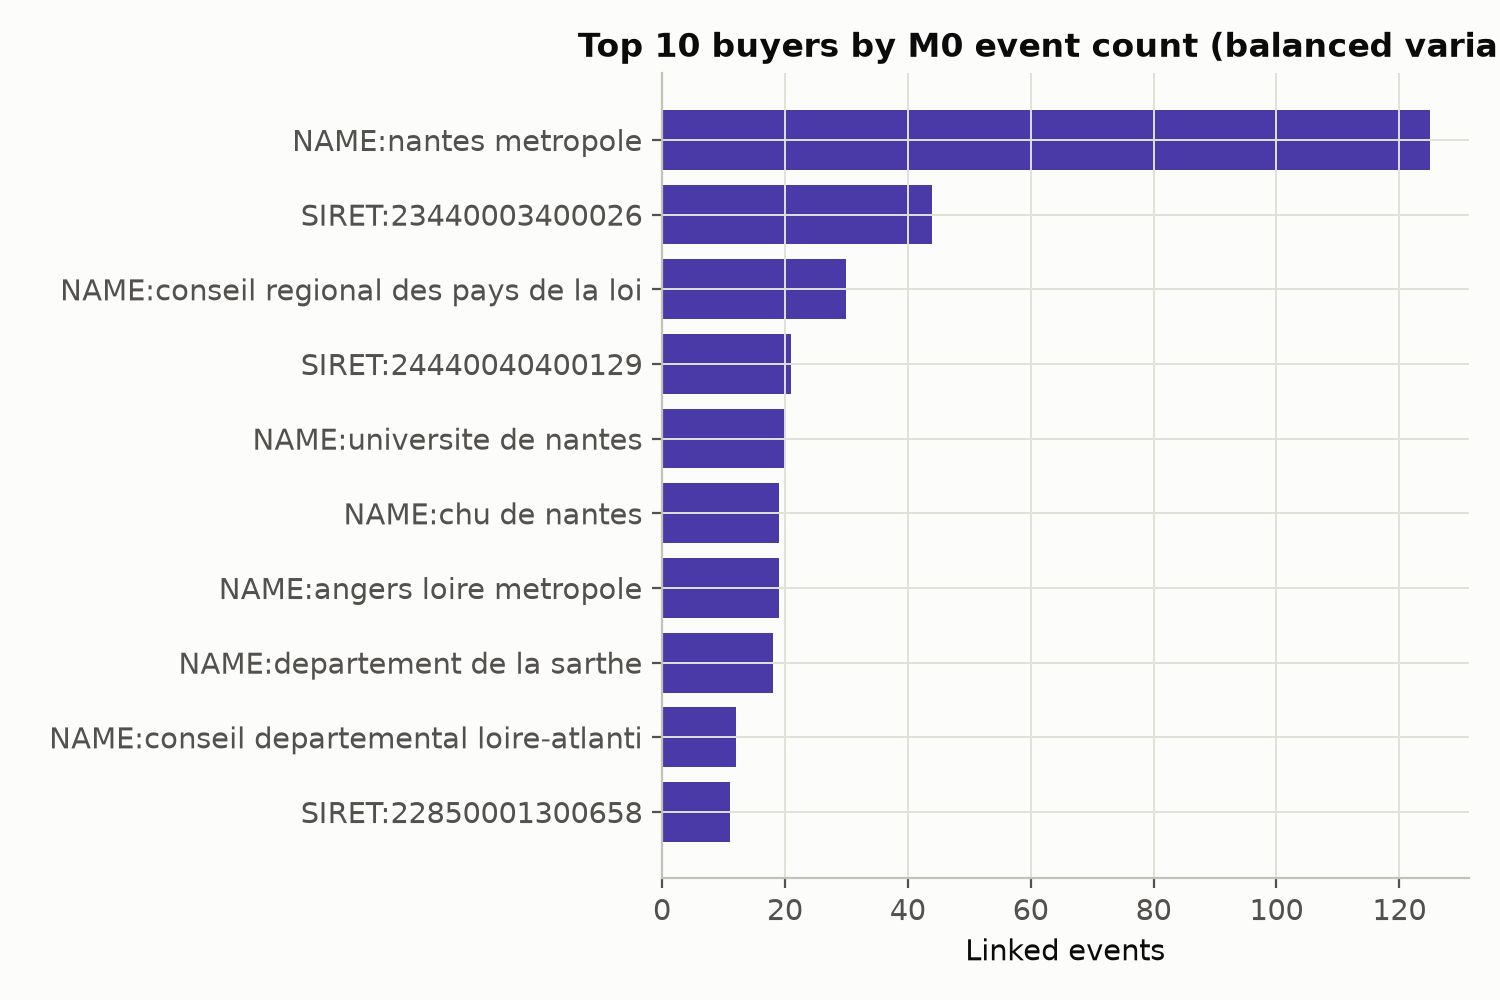
\includegraphics[width=0.8\linewidth]{10_top_buyer_event_counts.png}
\caption{Top 10 buyers by balanced-variant event count. The top buyer,
\texttt{NAME:nantes metropole}, contributes 125 of 618 events (20.2\%) ---
notably a name-keyed, not SIRET-keyed, buyer.}
\label{fig:topbuyers}
\end{figure}

\section{Worked Examples}
\label{sec:worked}

\subsection{Worked Link Example}
Source notice \texttt{15-139094} (SDIS de la Vend\'ee, buyer key
\texttt{NAME:sdis 85}) was published 2015-09-10, object ``\emph{Acquisition
d'appareils respiratoires isolants \`a circuit ouvert et de bouteilles
d'air pour le SDIS de la Vend\'ee \`a La Roche-sur-Yon}'' (self-contained
breathing apparatus), CPV \texttt{35111100} (division 35, class 3511,
category 35111). Its declared duration was missing and was imputed to 48
months (the division-35 observed median), giving
$\hat e = 2015\text{-}12\text{-}07 + 48\text{ mo} = 2019\text{-}12\text{-}07$.

Three same-buyer candidates fell inside the $\pm 6$-month window around
$\hat e$; their full scored rows, exactly as stored in
\texttt{boamp\_m0\_candidate\_pairs.csv}, are:

\begin{table}[h!]
\centering
\caption{Complete candidate pool for source \texttt{15-139094}
(\texttt{data/processed/boamp\_m0\_candidate\_pairs.csv}).}
\small
\begin{tabular}{lrrrrrrr}
\toprule
Candidate & Gap (mo) & $s_{\text{time}}$ & $s_{\text{text}}$ & $s_{\text{cpv}}$ & $s_{\text{buyer}}$ & $S(i,j)$ & Rank \\
\midrule
\texttt{19-141668} & 48.29 & 0.5675 & 0.1336 & 0.6 & 0.6 & \textbf{0.4286} & 1 \\
\texttt{20-72017} & 56.80 & 0.0145 & 0.3058 & 0.6 & 0.6 & 0.3507 & 2 \\
\texttt{19-108347} & 46.02 & 0.1897 & 0.0090 & 0.0 & 0.6 & 0.1106 & 3 \\
\bottomrule
\end{tabular}
\end{table}

The best-scoring candidate is \texttt{19-141668}, published
2019-09-19, object ``\emph{Acquisition d'un simulateur de feux r\'eels avec
traitement des fum\'ees destin\'e \`a la formation des sapeurs-pompiers du
SDIS de la Vend\'ee}'' (a fire-training simulator), CPV \texttt{35110000}
(division 35, class 3511, category 35110). Note how the pool illustrates
the scoring trade-offs: the rank-2 candidate actually has \emph{higher}
text similarity (0.306 vs.\ 0.134) but lands at the far edge of the
temporal window ($s_{\text{time}}=0.014$), while the rank-3 candidate is
temporally closer but nearly text-orthogonal and in a different CPV
division ($s_{\text{cpv}}=0$).

\begin{table}[h!]
\centering
\caption{Score calculation for the pair (\texttt{15-139094} $\rightarrow$
\texttt{19-141668}).}
\begin{tabular}{lll}
\toprule
Quantity & Formula / value & Result \\
\midrule
$t_j - t_i$ & gap in months & 48.29 \\
$|(t_j-t_i) - d_i|$ & $|48.29 - 48|$ & 0.29 \\
$s_{\text{time}}$ & $1 - 0.29/6$ & 0.5675 \\
$s_{\text{text}}$ & TF-IDF cosine of the two objects & 0.1336 \\
$s_{\text{cpv}}$ & same 4-digit class (3511), different 5-digit category & 0.6000 \\
$s_{\text{buyer}}$ & \texttt{NAME\_FALLBACK} & 0.6000 \\
$S(i,j)$ & $0.35(0.1336)+0.30(0.6)+0.25(0.5675)+0.10(0.6)$ & \textbf{0.4286} \\
\bottomrule
\end{tabular}
\end{table}
This pair had a margin of 0.078 over the second-best of 3 candidates and
was selected as source \texttt{15-139094}'s best match; because
$0.4286 \geq \tau_{\text{balanced}}=0.3230$ (and also $\geq
\tau_{\text{strict}}=0.3931$), the source is recorded as \texttt{event}=1
with \texttt{time\_to\_event\_or\_censor\_months}=48.29 in
\texttt{boamp\_survival\_m0\_balanced.csv}. Downstream, this row
contributes one event at $t=48.29$ months to the balanced Kaplan--Meier
curve of Figure~\ref{fig:kmoverall}, one uncensored observation to the
division-35 stratum in Figure~\ref{fig:kmcpv}, and one
\texttt{dur\_was\_imputed}=\texttt{True} event to the Cox model of
Section~\ref{sec:cox} --- and, because its 48-month duration was itself
imputed, it is also a concrete instance of the duration-circularity
mechanism audited in Section~\ref{sec:leakage}: the imputed duration
placed the search window that found the candidate that became the event.
This example is instructive precisely because the text score is low
(0.134, well below the accepted-link mean of 0.305): the link survives on
the combination of CPV-class agreement and near-exact temporal alignment
with the (imputed) expected end date, illustrating why the composite
design --- rather than a single dominant signal --- matters, but also why
low-text-similarity links deserve scrutiny in manual review
(Section~\ref{sec:manual}).

\subsection{Worked Censoring Example}
Source notice \texttt{24-10209} (SEMITAN, Nantes's public transport
operator, buyer key \texttt{NAME:semitan}) was published 2024-01-29, object
``\emph{Renouvellement des infrastructures Serveurs - Licences Vmware}''
(server infrastructure and VMware license renewal), CPV \texttt{72212218}
(division 72, IT services). Its declared duration was \emph{directly
observed} (not imputed) at 36 months, giving $\hat e = 2027\text{-}01\text{-}29$.

SEMITAN is a frequent buyer with 32 digital AO sources across the study
period, so this is not a case of ``no later same-buyer notice'' --- indeed
six further SEMITAN notices were published in 2024--2025 alone. But the
$\pm 6$-month candidate window around $\hat e$ spans only
2026-07-29--2027-07-29, and the latest SEMITAN notice observed in the
corpus (\texttt{25-97524}, 2025-09-02) still falls nearly a year before
that window opens. The source therefore has \emph{zero} candidates ---
the ``temporal-window-excluded'' failure mode of
Section~\ref{sec:diagnostics} --- and is recorded as \texttt{event}=0 with
\texttt{time\_to\_event\_or\_censor\_months} $=$ (2026-07-13
$-$ 2024-01-29) $\approx$ 29.4 months. In survival language, the only valid
statement is ``no recurrence was detected by month 29.4 under the current
$\pm 6$-month window''; it is neither evidence that SEMITAN will not
re-tender this need, nor evidence that it will.

\section{Limitations and Risks}
\label{sec:limitations}

\begin{description}
\item[L1. No ground truth.] BOAMP provides no renewal field; the M0 event
is entirely a constructed proxy. Precision/recall are only estimated
indirectly (Section~\ref{sec:fs}) and not yet validated against manual
labels (Section~\ref{sec:manual}).
\item[L2. Blocking, not scoring, is the binding constraint.] 60.9\% of
eligible sources never enter the candidate universe $\Omega$
(Section~\ref{sec:blocking}); this ceiling cannot be moved by tuning score
weights or thresholds.
\item[L3. Duration circularity.] Declared/imputed duration constructs the
estimated end date used for blocking \emph{and} temporal scoring, and
duration remains available downstream as a survival covariate. The
estimated duration hazard-ratio sign is not stable to alternative,
duration-independent linkage designs (Section~\ref{sec:leakage}).
\item[L4. Name-fallback buyer fragmentation.] 77.4\% of M0 sources are
name-keyed; no fuzzy-name or external-registry reconciliation is
implemented, so buyer-name variants split into separate groups and produce
structural false negatives.
\item[L5. Candidate reuse.] 27.3\% of accepted balanced-link candidates are
claimed as the best match by more than one source (max.\ multiplicity 6),
which is not automatically an error (lots, frameworks) but prevents a naive
one-to-one interpretation without manual review.
\item[L6. Sample scope.] The dataset covers only Pays de la Loire,
digital/ICT contracts, 2015--2026. Linking rates, score distributions, and
CPV-division rankings may differ substantially elsewhere.
\item[L7. Sparse survival covariates.] The Cox model's CPV-division dummy
structure produces convergence/separation warnings for rare divisions
(Section~\ref{sec:cox}), and temporal (train/test) validation was attempted
but deferred as unstable (Section~\ref{sec:sensitivity}).
\end{description}

\section{Dataset Reliability Checks}
\label{sec:reliability}

\subsection{Confidence Tiers}
Because \texttt{strict} $\subset$ \texttt{balanced} $\subset$
\texttt{broad} (Section~\ref{sec:algo}), the three named thresholds
naturally partition the 927 broad-linked sources into three confidence
tiers of near-identical size (each spans a 25-percentile-point band of the
rank-1 score distribution):

\begin{table}[h!]
\centering
\caption{Confidence tiers derived from the nested broad/balanced/strict
thresholds.}
\label{tab:tiers}
\begin{tabular}{lrl}
\toprule
Tier & Count & Composite-score band \\
\midrule
HIGH (= strict set) & 309 & $S \geq 0.3931$ \\
MEDIUM (balanced minus strict) & 309 & $0.3230 \leq S < 0.3931$ \\
LOW (broad minus balanced) & 309 & $0.2642 \leq S < 0.3230$ \\
\midrule
Not linked even at broad threshold & 927 (of 1{,}236 blocked) & $S < 0.2642$ \\
Blocked, zero candidates & 1{,}923 & N/A \\
\bottomrule
\end{tabular}
\end{table}
The reference (balanced) event set is HIGH $\cup$ MEDIUM (618 sources).
Restricting further to HIGH-only (strict, 309 events) is the conservative
sensitivity check used throughout Section~\ref{sec:sensitivity}.

\subsection{Unsupervised Fellegi--Sunter Latent-Mixture Diagnostic}
\label{sec:fs}
Following the latent-class reading of the Fellegi--Sunter model
\cite{fellegi1969}, in which match ($M$) and non-match ($U$) parameters can
be estimated without labeled data via the EM algorithm
\cite{dempster1977,winkler1988}, an unsupervised two-class Beta mixture
(match class $M$, non-match class $U$) was fitted by EM over the comparison
vectors
$\gamma_j=(s_{\text{text}},s_{\text{cpv}},s_{\text{time}},s_{\text{buyer}})$
of \emph{all} 6{,}137 pairs in $\Omega$, not only rank-1 winners
(Figure~\ref{fig:betamix}). This is a model-based internal diagnostic, not
external validation: \texttt{s\_cpv} is discrete and \texttt{s\_buyer} is
nearly source-level rather than pair-level, both approximated by continuous
Beta densities. EM converged to log-likelihood 40{,}975.5 (identical across
warm-start and 6 total restarts, Jaccard=1.0 on posteriors $>0.5$),
estimated mixing weight $\hat p = 0.181$.

For posterior match probability $r_j = P(M \mid \gamma_j)$:
\begin{equation}
\widehat{\text{precision}}_{\text{FS}} = \frac{\sum_{j \in L_{\text{balanced}}} r_j}{|L_{\text{balanced}}|} = 0.455,
\qquad
\widehat{\text{recall}}_\Omega = \frac{\sum_{j \in L_{\text{balanced}}} r_j}{\sum_{j \in \Omega} r_j} = 0.253.
\end{equation}
$\widehat{\text{recall}}_\Omega$ is conditional on $\Omega$ and explicitly
excludes the 1{,}923 zero-candidate sources; it cannot be read as recall
over all possible true recurrences. A conditional-independence check between
the two continuous components found weak correlation (Pearson
$r=0.047$ between \texttt{s\_cpv} and \texttt{s\_text} on the 618 linked
pairs, Spearman $r=-0.106$, both below the 0.3 flag threshold), supporting
--- but not proving --- the model's conditional-independence assumption.

\begin{figure}[h!]
\centering
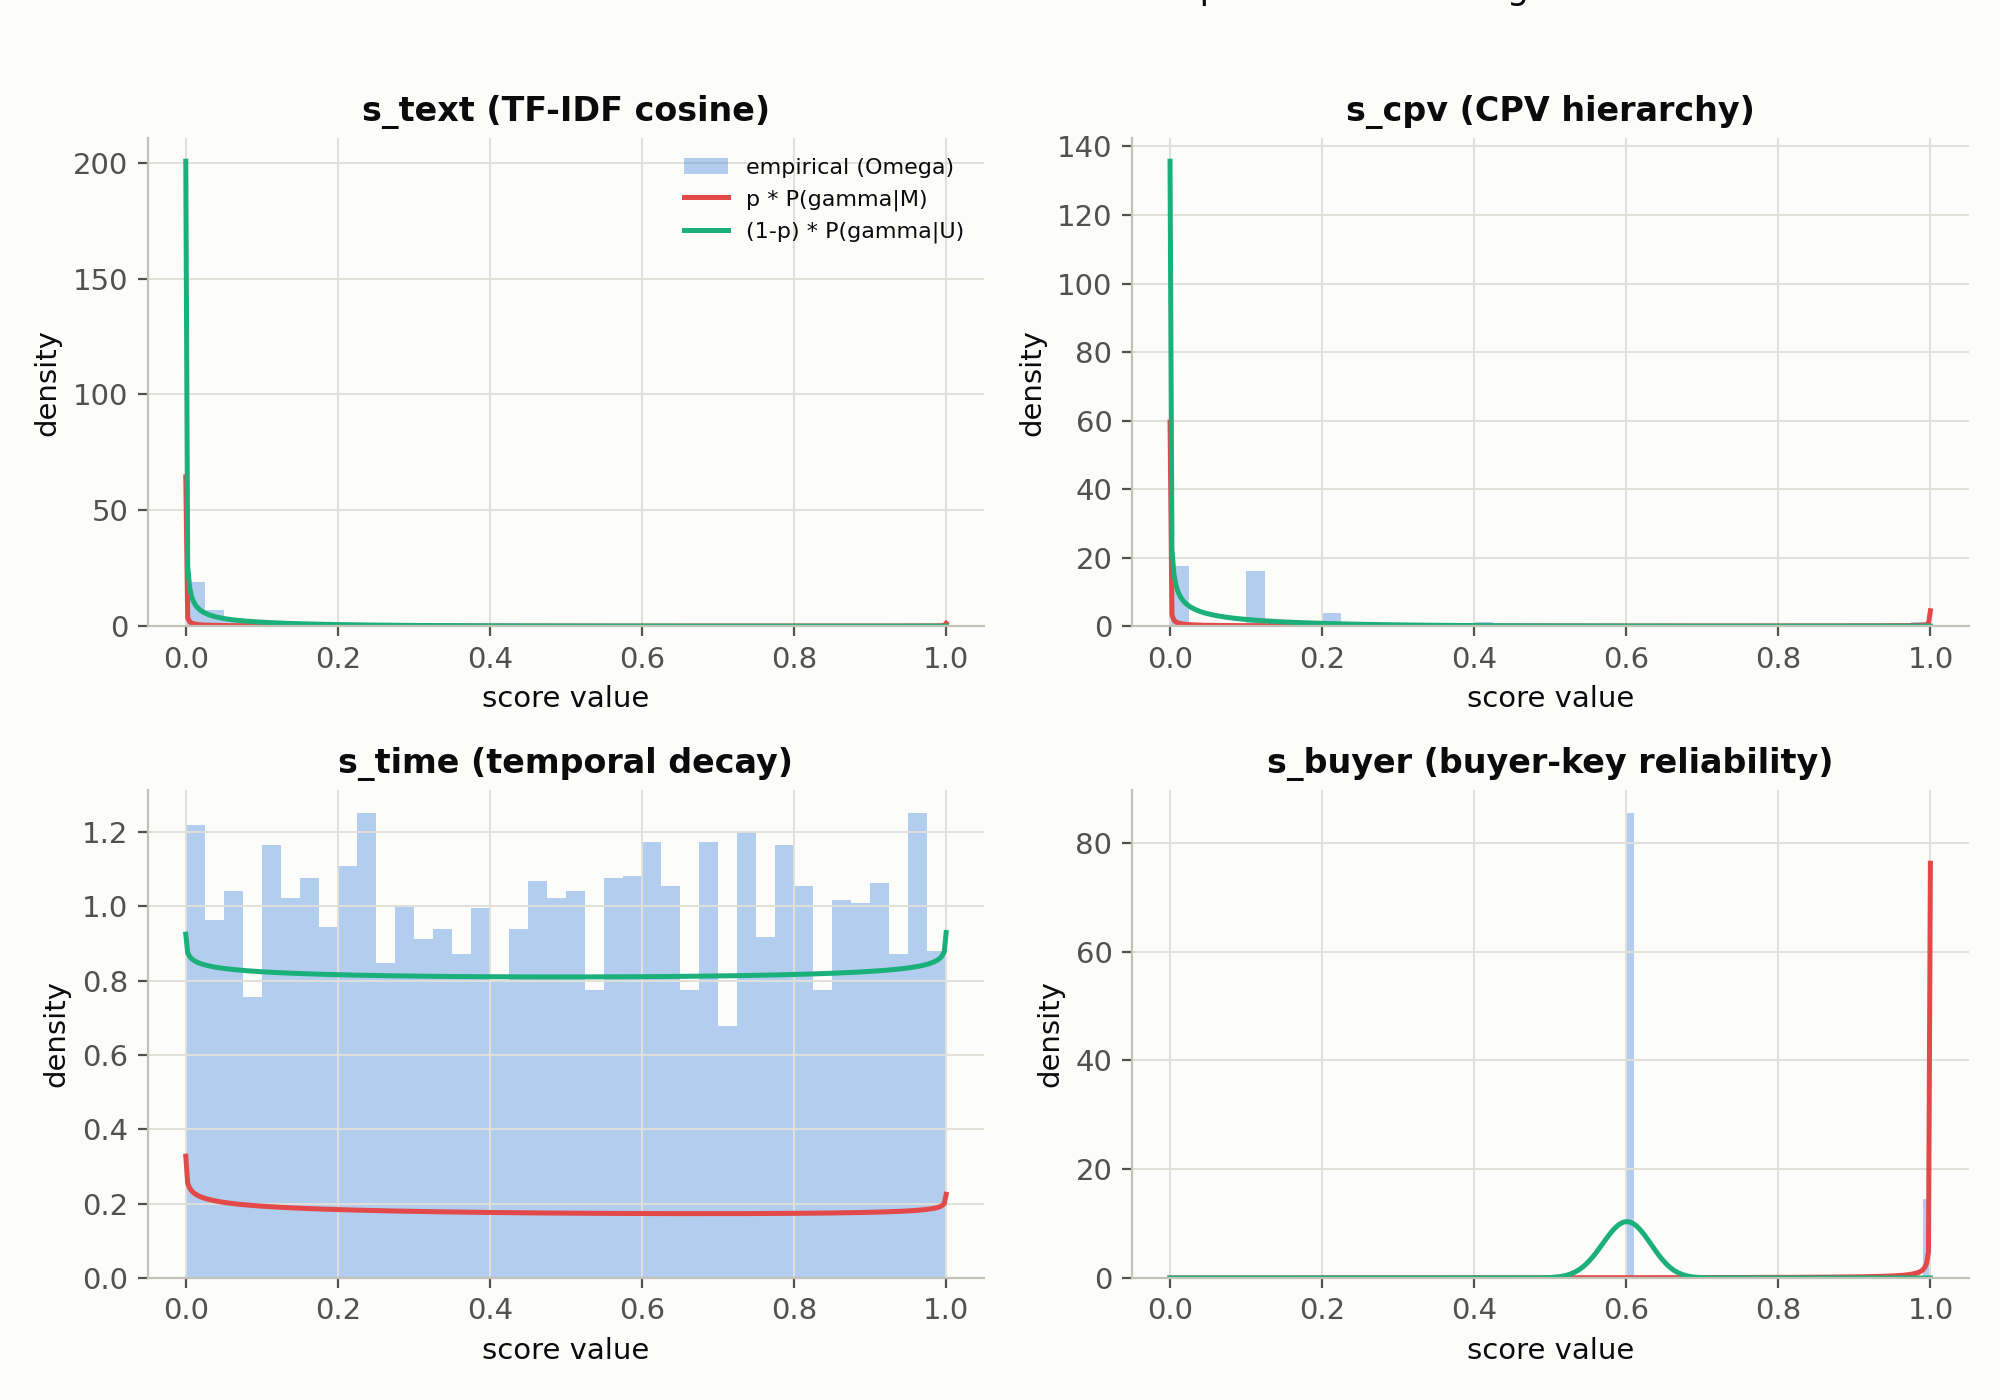
\includegraphics[width=\linewidth]{11_beta_mixture_densities.png}
\caption{Fitted Beta-mixture densities ($p\cdot P(\gamma\mid M)$ in red,
$(1-p)\cdot P(\gamma\mid U)$ in aqua) against empirical score histograms,
for each of the four score components over $\Omega$ ($n=6{,}137$ pairs).}
\label{fig:betamix}
\end{figure}

\begin{figure}[h!]
\centering
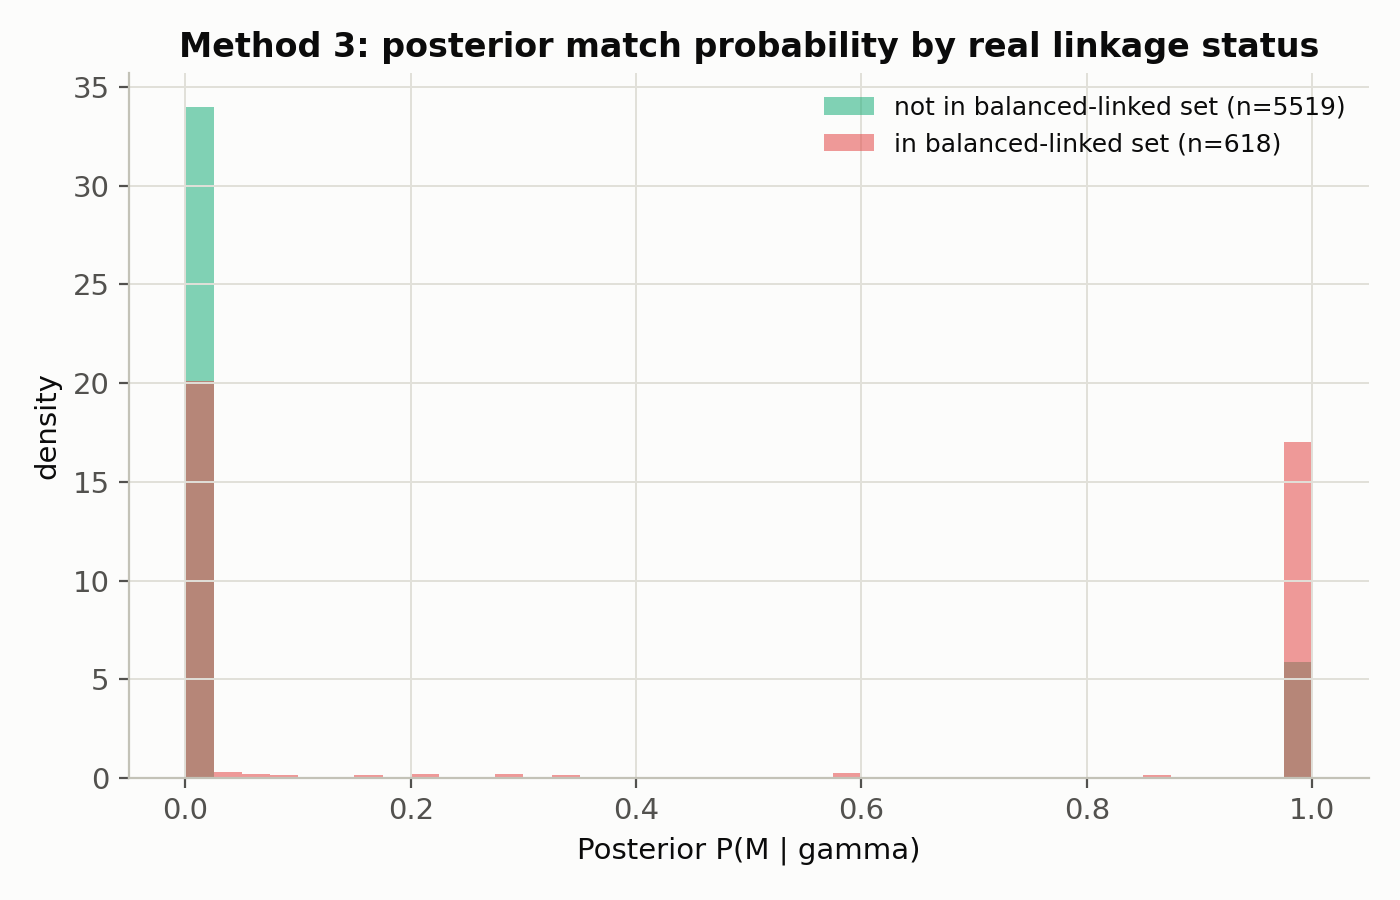
\includegraphics[width=0.75\linewidth]{12_beta_mixture_posterior_by_linkage.png}
\caption{Posterior match probability $P(M\mid\gamma)$, split by whether the
pair is in the balanced-linked set. The two distributions separate but
overlap substantially, consistent with the moderate model-based precision
estimate above.}
\label{fig:betapost}
\end{figure}

\subsection{Semi-Synthetic Corruption Recovery}
Using the 309 strict links as a conservative (not ground-truth) reference
subset, text/CPV/duration fields were corrupted at increasing severity
levels 0--3; a pair is ``recovered'' if the true candidate remains top-ranked
in its (fixed) real candidate pool and still clears the balanced threshold.

\begin{table}[h!]
\centering
\caption{Recovery rate $R(\text{severity})$ under semi-synthetic corruption
(\texttt{reports/tables/m4\_recovery\_summary.csv}), $n=309$.}
\begin{tabular}{lrrrrr}
\toprule
Sweep & $R_0$ & $R_1$ & $R_2$ & $R_3$ & $R_0 - R_3$ \\
\midrule
Combined & 1.000 & 0.906 & 0.654 & 0.524 & 0.476 \\
Text only & 1.000 & 0.916 & 0.777 & 0.718 & 0.282 \\
CPV only & 1.000 & 0.990 & 0.984 & 0.851 & 0.149 \\
Duration only & 1.000 & 0.987 & 0.864 & 0.981 & 0.019 \\
\bottomrule
\end{tabular}
\end{table}

\begin{figure}[h!]
\centering
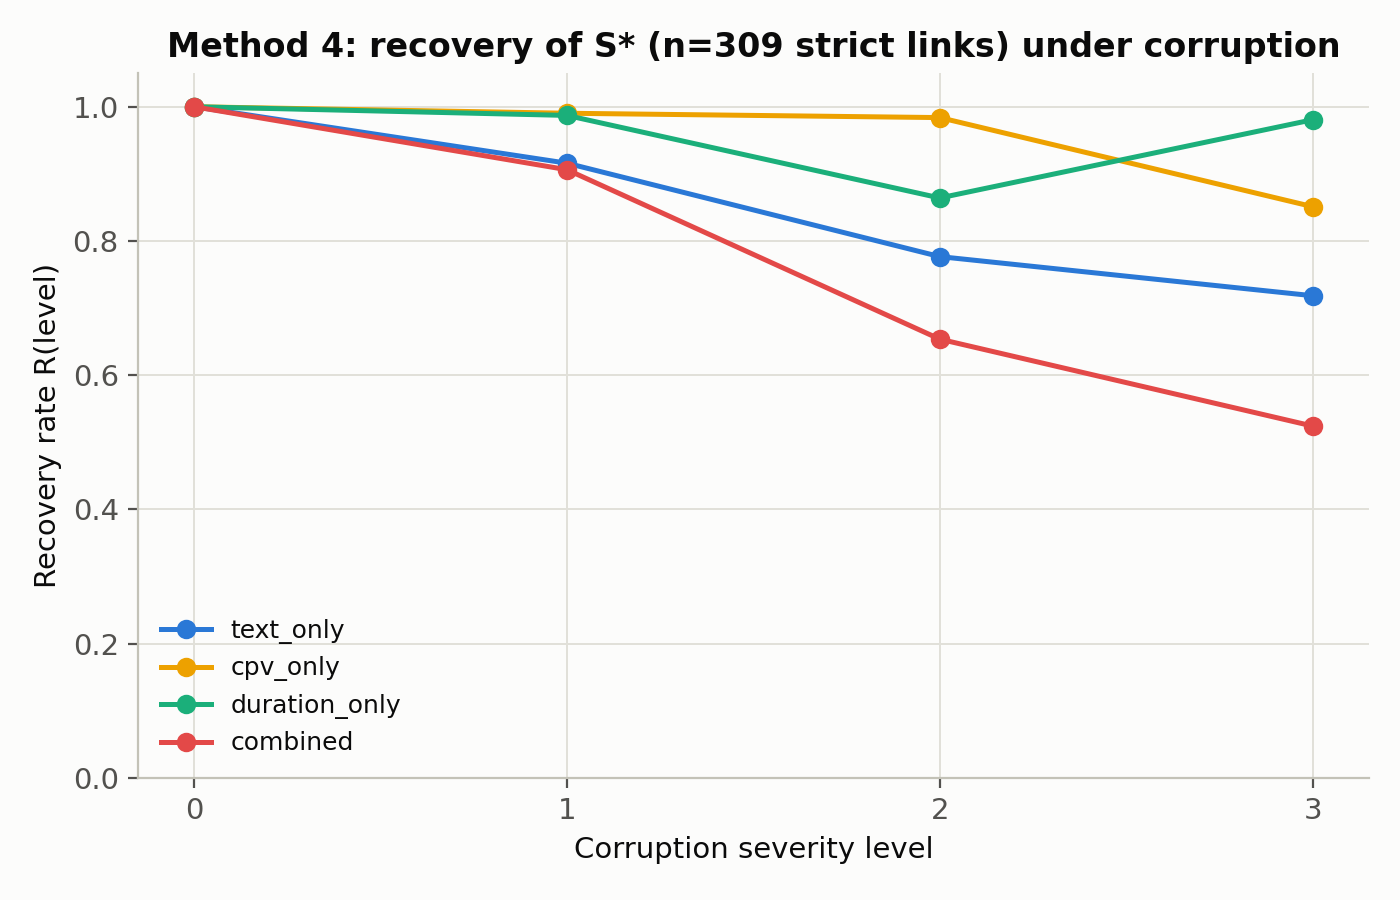
\includegraphics[width=0.75\linewidth]{13_corruption_recovery_curves.png}
\caption{Recovery rate of the true strict-link candidate under increasing
per-field corruption severity, by which field is corrupted.}
\label{fig:corruption}
\end{figure}
Text degradation is the main breaking point; duration-only corruption is
unusually robust because most strict-link sources already carry imputed
durations close to their CPV-division median, so perturbing an already-imputed
value changes little. This experiment holds the candidate pool fixed and so
does \emph{not} test corruption effects that would alter blocking itself
--- a full reblocking corruption study remains deferred (Section~\ref{sec:manual}).

\subsection{Statistical Roadmap}
Table~\ref{tab:roadmap} separates the different roles these tools play,
following the credibility-audit discipline that a statistically significant
result is not the same as a good ranking metric, and a stable internal
diagnostic is not external validation.

\begin{table}[h!]
\centering
\caption{Statistical roadmap for this report.}
\label{tab:roadmap}
\small
\begin{tabular}{p{0.16\textwidth}p{0.1\textwidth}p{0.32\textwidth}p{0.32\textwidth}}
\toprule
Tool & Type & Question answered & Main limitation \\
\midrule
Fellegi--Sunter mixture & Model-based estimator & Model-based precision/recall on $\Omega$? & Conditional on blocking; not verified accuracy. \\
Corruption recovery & Semi-synthetic diagnostic & Robustness of strict links to field degradation? & Fixed candidate pool; does not test reblocking. \\
Threshold sensitivity & Sensitivity sweep & How many links flip near $\tau_{\text{balanced}}$? & Describes ambiguity, not correctness. \\
Feature ablation & Sensitivity sweep & Which component drives the ranking? & Score-internal; not validated against labels. \\
Kaplan--Meier & Estimator & Time-to-linked-recurrence distribution? & Estimates the proxy event's timing, not legal renewal. \\
Cox PH model & Regression & Which covariates associate with the proxy hazard? & Associations conditional on the constructed event; not causal. \\
Duration-leakage audit & Design-sensitivity check & Is the duration effect robust to linkage design? & Answer here is \emph{no} (Section~\ref{sec:leakage}). \\
\bottomrule
\end{tabular}
\end{table}

\section{Survival Analysis: Methods}
\label{sec:survival-methods}

\subsection{Dataset Overview}
\begin{table}[h!]
\centering
\caption{Reference survival dataset summary
(\texttt{boamp\_survival\_m0\_balanced.csv}).}
\begin{tabular}{lr}
\toprule
Metric & Value \\
\midrule
Total sources (rows) & 3{,}159 \\
Events (\texttt{event}=1) & 618 (19.6\%) \\
Censored (\texttt{event}=0) & 2{,}541 (80.4\%) \\
Study period & 2015-03-02 to 2026-07-13 \\
Median linked gap (events only) & 37.7 months \\
\bottomrule
\end{tabular}
\end{table}

\subsection{Notation and Methods}
Let $T_i^{\text{obs}} = \min(T_i, C_i)$ and $\delta_i = \mathbf 1[T_i \leq
C_i]$, stored as \texttt{time\_to\_event\_or\_censor\_months} and
\texttt{event}.

\textbf{Kaplan--Meier estimator} \cite{kaplan1958}. $\hat S(t) =
\prod_{j:t_j\leq t}(1 - d_j/n_j)$, the probability of not-yet-linked
survival past $t$, where $n_j$ is the number at risk just before event time
$t_j$ and $d_j$ the number of events at $t_j$. Its validity as an unbiased
estimator requires censoring to be non-informative --- an assumption that
is \emph{not} guaranteed here, since censoring mixes administrative
end-of-study with linkage failure (blocking exclusion, sub-threshold
scores); the censoring-balance diagnostic in
\texttt{audit\_censoring\_diagnostics.csv} shows censored sources differ
systematically from event sources (e.g.\ far fewer scored candidates and
lower buyer publication frequency), so KM curves must be read as
descriptive summaries of the constructed proxy process, not as unbiased
estimates of a well-defined recurrence-time distribution.

\textbf{Restricted mean survival time (RMST)} at horizon $\tau=60$ months,
$\int_0^{\tau}\hat S(t)\,dt$ --- the model-free ``average event-free months
out of the first 60'' summary recommended when the median is not reached
\cite{royston2013} --- is used as the primary summary statistic
\emph{instead of} the median whenever $\hat S(t)$ never crosses 0.5 within
the observed range (which is the case for every variant in this study,
Section~\ref{sec:results}).

\textbf{Cox proportional hazards model} \cite{cox1972}: $h(t\mid \mathbf
x_i) = h_0(t) \exp(\boldsymbol\beta^\top \mathbf x_i)$, fit with
\texttt{lifelines} \cite{davidsonpilon2019} (penalizer $=0.01$), with
covariates log(1 + declared duration months),
the duration-imputation flag, CPV-division dummies, and buyer-key-type
dummies, and robust standard errors clustered by \texttt{buyer\_key} (a source contract
and its own linked candidate never share a cluster, but two different
sources from the same buyer do, and buyer-level clustering accounts for
that dependence). Hazard ratio $\mathrm{HR}_k = \exp(\beta_k)$; $>1$ means a
higher instantaneous linking rate (faster proxy recurrence).

\textbf{Proportional-hazards diagnostic}: scaled-Schoenfeld-residual test
($H_0$: PH holds) \cite{grambsch1994} via \texttt{lifelines}'
\texttt{check\_assumptions}.

\textbf{Parametric AFT models}: Weibull and log-normal accelerated
failure-time models, same covariate set, compared by AIC (lower is a better
fit/complexity trade-off among models on the same data) and in-sample
concordance.

\textbf{Functional form check}: a quadratic term
$(\log(1+d))^2$ added to the clustered Cox model, to test whether the
duration effect is linear on the log-hazard scale.

\textbf{Prediction calibration}: for horizons $h\in\{12,24\}$ months,
predicted risk $1-\hat S(h\mid \mathbf x_i)$ from the fitted Cox model is
grouped into quintiles and compared against the observed
$\mathbf 1[\texttt{event}=1 \wedge T^{\text{obs}} \leq h]$ rate and Brier
score \cite{brier1950} per quintile.

All of the above are refit on eight event definitions (reference balanced,
broad, strict, and five duration/window sensitivity designs) to test
robustness (Section~\ref{sec:sensitivity}).

\section{Survival Results}
\label{sec:results}

\subsection{Kaplan--Meier Survival Estimates}
Figure~\ref{fig:kmoverall} shows the overall KM curve for all three named
variants. \textbf{None of the three curves cross 50\% survival}: median
survival is undefined (\texttt{inf}) for broad, balanced, and strict alike,
so RMST at 60 months is the primary descriptive summary
(Table~\ref{tab:kmoverall}).

\begin{figure}[h!]
\centering
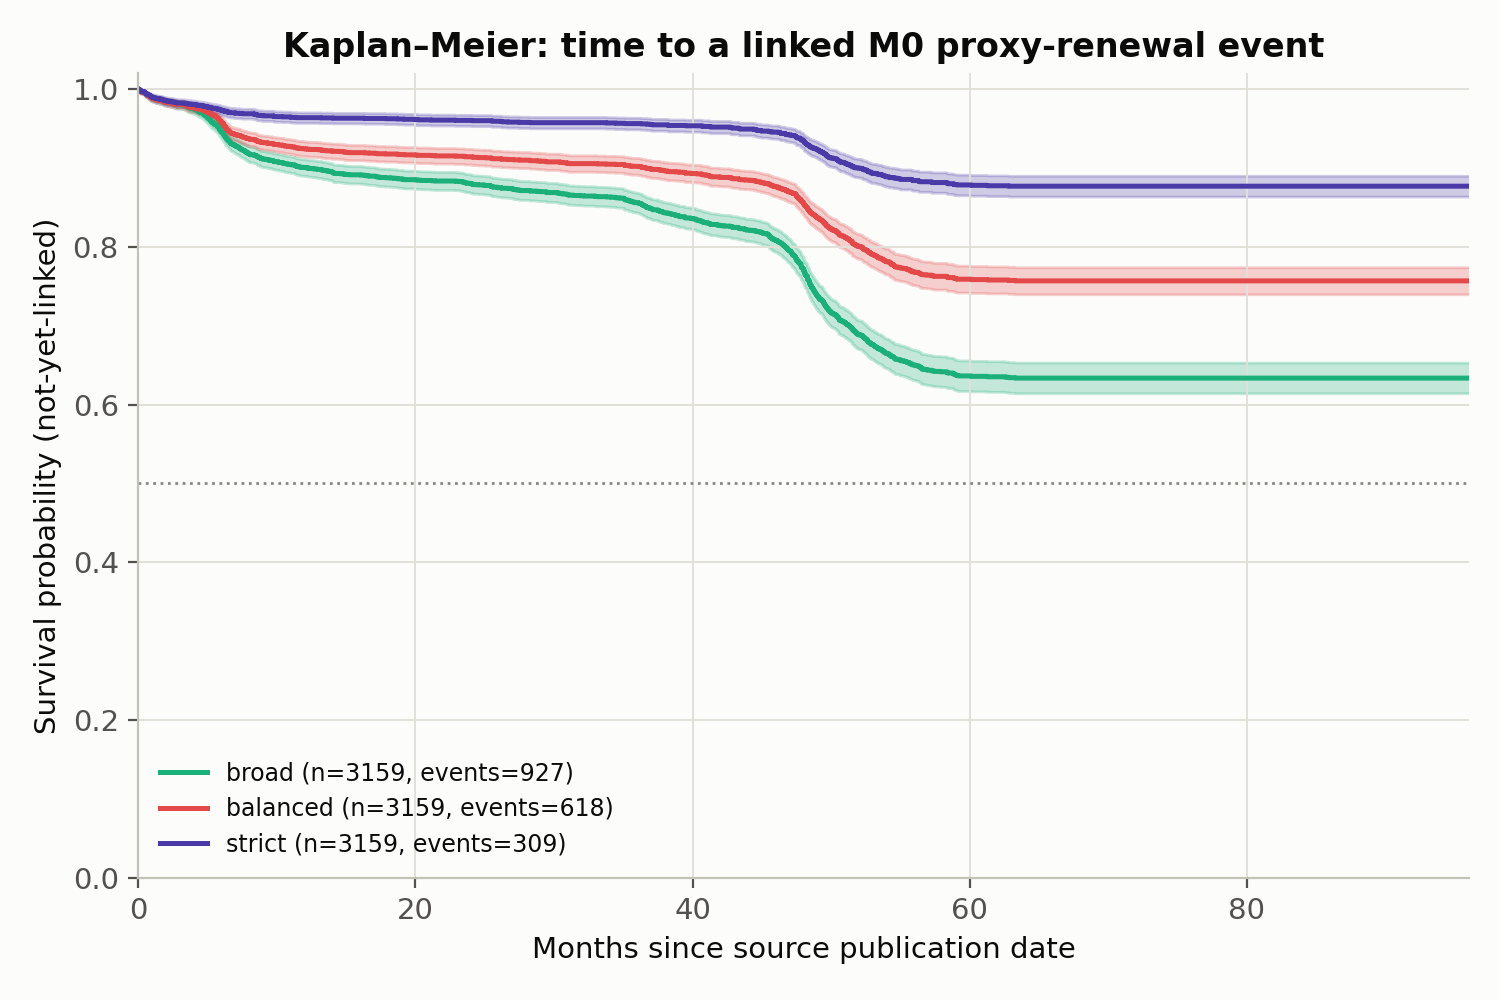
\includegraphics[width=0.85\linewidth]{17_km_overall_variants.png}
\caption{Kaplan--Meier survival curves (time to a linked M0 proxy-recurrence
event) for the three named threshold variants, with pointwise 95\%
confidence bands. The dotted line marks the 50\% level, which no curve
reaches within the observed follow-up.}
\label{fig:kmoverall}
\end{figure}

\begin{table}[h!]
\centering
\caption{Overall survival summary by variant
(\texttt{reports/tables/survival\_km\_summary.csv}).}
\label{tab:kmoverall}
\begin{tabular}{lrrrrr}
\toprule
Variant & Events & Censoring & Median & $S(24\text{mo})$ & RMST 60mo \\
\midrule
Broad & 927 & 70.7\% & undefined & 0.880 & 50.5 mo \\
\textbf{Balanced} & \textbf{618} & \textbf{80.4\%} & \textbf{undefined} & \textbf{0.914} & \textbf{53.5 mo} \\
Strict & 309 & 90.2\% & undefined & 0.960 & 56.9 mo \\
\bottomrule
\end{tabular}
\end{table}

\subsection{Kaplan--Meier by CPV Division}
Figure~\ref{fig:kmcpv} stratifies by the four core digital CPV divisions
under both the broad and strict variants. Ranking is \emph{not} stable
across variants: division 32 (telecommunications equipment) ranks
fastest-recurring (lowest RMST, 54.7 mo) under broad but slowest under
strict, and the Spearman correlation between the broad and strict RMST
rankings over the four core divisions is $\rho = -0.40$ ($p=0.60$, $n=4$;
\texttt{reports/tables/m6c\_km\_rank\_correlation.csv}) --- with only four
divisions this test has essentially no power, but the observed
\emph{negative} point estimate is enough to rule out treating the ranking
as stable. Division 72 (IT services) --- the largest single division by
volume (889 sources) --- ranks consistently mid-to-low. A
formal pairwise log-rank comparison across CPV divisions was attempted in
this run but produced no usable output rows (a type-mismatch between the
survival file's numeric-like \texttt{cpv\_division} values and the
comparison script's string literals, an implementation defect flagged
here rather than silently worked around); the KM/RMST comparison below is
therefore the descriptive substitute for a formal test in the current run.

\begin{figure}[h!]
\centering
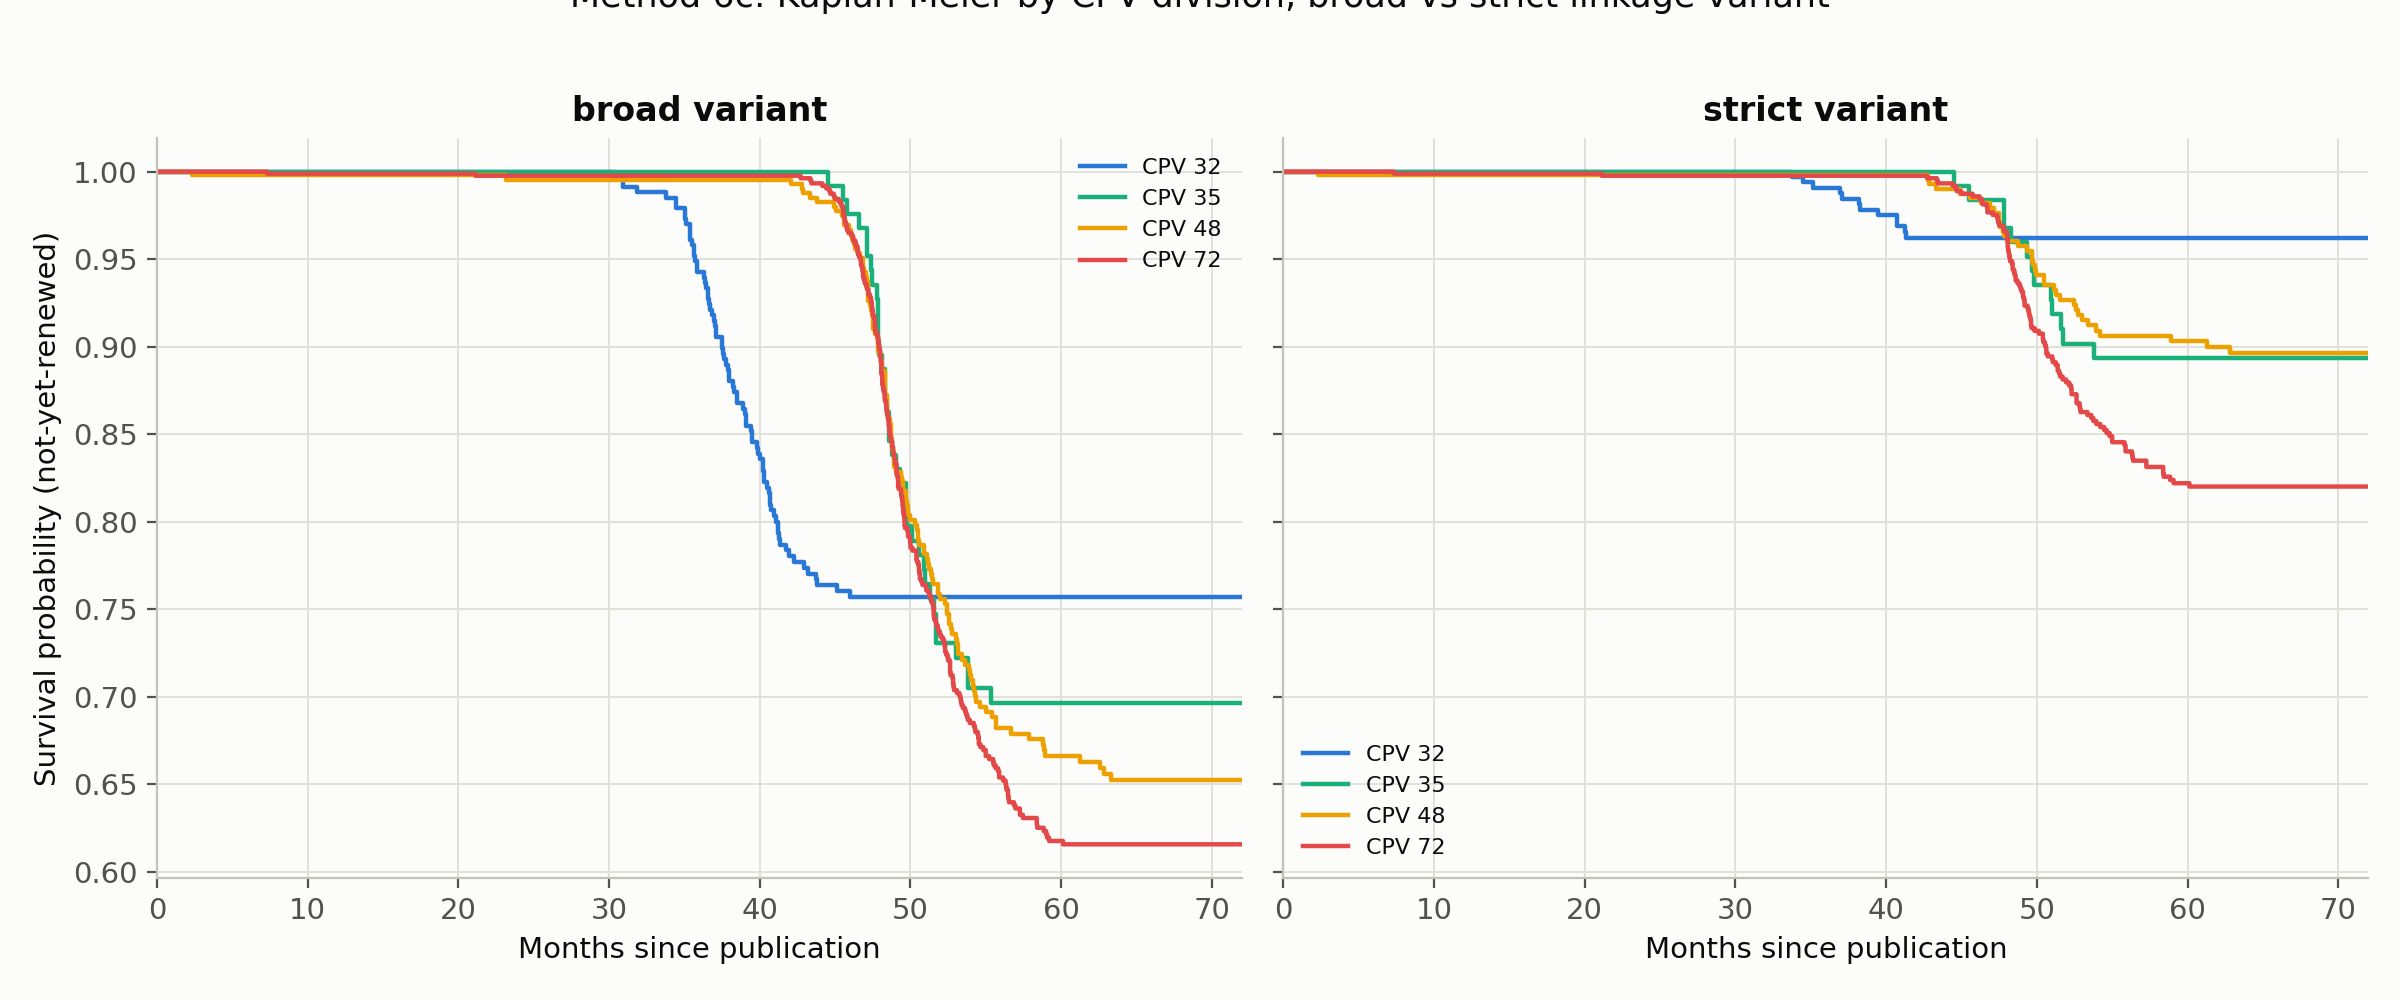
\includegraphics[width=\linewidth]{16_km_by_cpv_division_broad_vs_strict.png}
\caption{Kaplan--Meier by CPV division, broad (left) vs.\ strict (right)
variant. Ranking instability across variants argues against confirmatory
segment-level claims.}
\label{fig:kmcpv}
\end{figure}

\subsection{Cox Proportional Hazards Model}
\label{sec:cox}
Table~\ref{tab:coxnoncpv} reports the interpretable, non-CPV terms of the
buyer-clustered Cox model fit on the balanced reference event definition
($n=3{,}159$, 618 events); Figure~\ref{fig:coxforest} plots the same terms
as hazard ratios. The full model also includes 31 CPV-division dummy terms
(\texttt{reports/tables/survival\_cox\_models.csv}); several fire with
extreme coefficients on sparse divisions (e.g.\ division 33 with only 10
sources, HR$=21.3$, or division 43 with a single source, HR$\approx 0$),
a documented symptom of separation in small strata rather than a credible
substantive effect --- this is itself a finding (Section~\ref{sec:limitations},
L7), not a result to be read at face value.

\begin{table}[h!]
\centering
\caption{Balanced clustered Cox model, non-CPV terms
(\texttt{reports/tables/survival\_cox\_models.csv}).}
\label{tab:coxnoncpv}
\begin{tabular}{lrrr}
\toprule
Term & HR & 95\% CI & $p$ \\
\midrule
$\log(1+\text{declared duration, months})$ & 0.923 & [0.771, 1.105] & 0.384 \\
Duration was imputed (ref.\ observed) & \textbf{0.433} & [0.280, 0.670] & \textbf{$<$0.001} \\
Buyer key = RAW\_SIRET (ref.\ NAME\_FALLBACK) & 1.224 & [0.631, 2.375] & 0.549 \\
\bottomrule
\end{tabular}
\end{table}

\begin{figure}[h!]
\centering
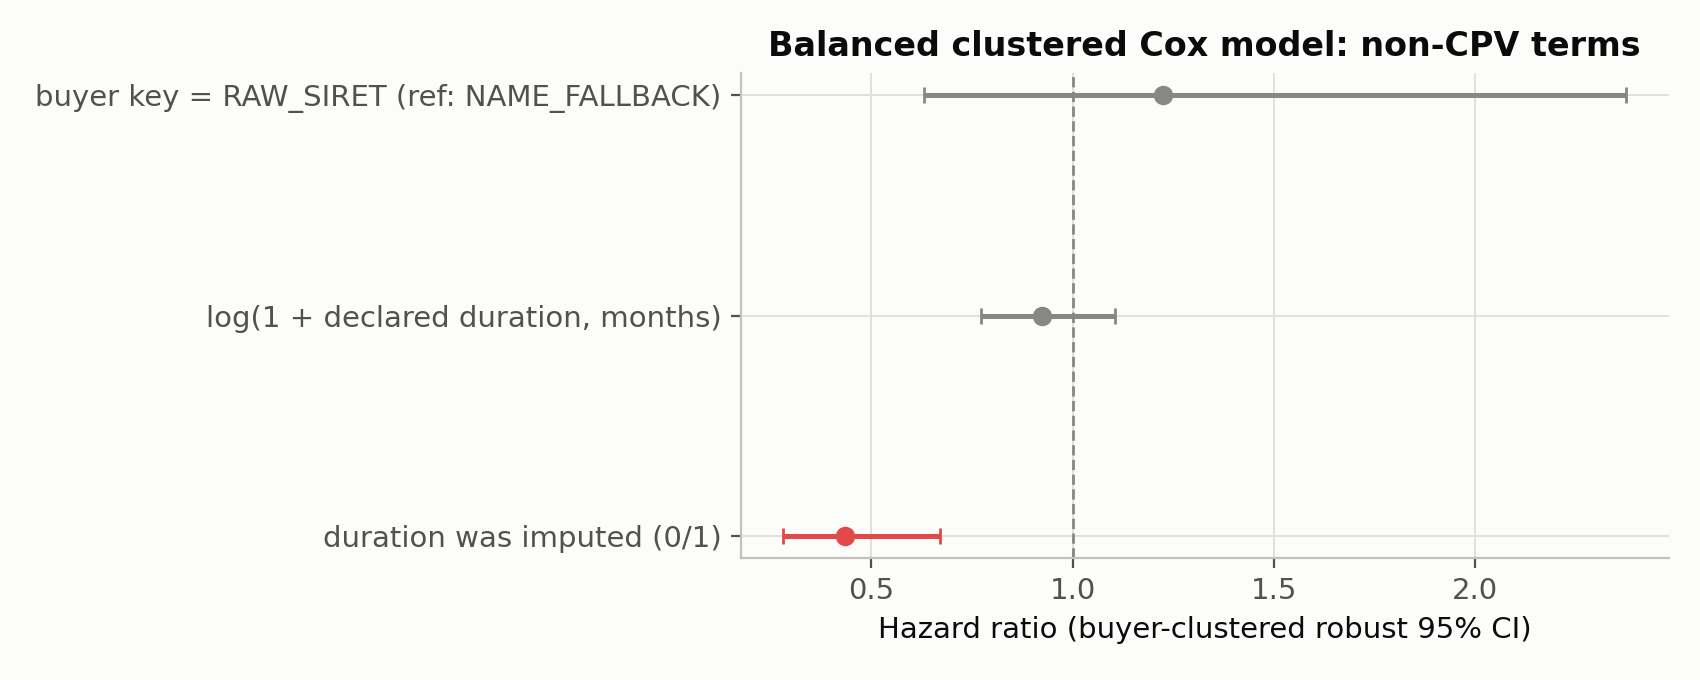
\includegraphics[width=0.85\linewidth]{18_cox_forest_balanced_noncpv.png}
\caption{Forest plot of the balanced clustered Cox model's non-CPV hazard
ratios (buyer-clustered robust 95\% CI). Red marks the term significant at
5\%.}
\label{fig:coxforest}
\end{figure}

The only term reaching conventional significance is
\texttt{dur\_was\_imputed}: sources whose duration had to be imputed show a
\emph{lower} instantaneous linking hazard (HR$=0.433$) than sources with an
observed duration. Given that imputation defaults to a CPV-division median
--- which mechanically widens or shifts the $\pm 6$-month blocking window
relative to a source's true (unknown) contract length --- this is at least
as plausibly a \emph{linkage-design artifact} as a substantive difference
in recurrence behavior, and should not be reported as a business finding
without the leakage caveats of Section~\ref{sec:leakage}. Declared duration
itself is small and not significant in this design (HR$=0.923$, $p=0.38$);
Section~\ref{sec:leakage} shows this coefficient is unstable in sign and
magnitude across alternative linkage designs.

\subsection{Proportional-Hazards and Functional-Form Diagnostics}
The Schoenfeld residual test on the balanced model flags four terms at
$p<0.05$: \texttt{log\_duration} ($p=6.8\times10^{-6}$),
\texttt{dur\_was\_imputed} ($p=7.7\times10^{-4}$), \texttt{cpv\_division\_72}
($p=7.3\times10^{-5}$), and \texttt{cpv\_division\_MISSING} ($p=0.042$)
(\texttt{reports/tables/survival\_ph\_diagnostics\_balanced.csv}). The
duration-related flags are consistent with the functional-form check: adding
a quadratic $(\log(1+d))^2$ term to the clustered Cox model gives HR$=1.010$
($p=0.365$) for the quadratic term itself while the linear term drops to
HR$=0.992$ ($p=0.899$) --- i.e.\ once duration and the duration-imputation
flag are both in the model, most of the apparent duration signal is not
well described by a simple linear log-hazard term, and should be read as an
average effect over the observation window rather than a constant
month-by-month multiplier.

\subsection{Parametric AFT Models}
\begin{table}[h!]
\centering
\caption{Parametric AFT model comparison, balanced reference
(\texttt{reports/tables/survival\_aft\_models.csv}).}
\begin{tabular}{lrrr}
\toprule
Model & AIC & Log-likelihood & Concordance \\
\midrule
Weibull AFT & 8{,}059.8 & $-$3{,}990.9 & 0.7135 \\
\textbf{Log-normal AFT} & \textbf{7{,}948.96} & $\mathbf{-3{,}935.5}$ & \textbf{0.7248} \\
\bottomrule
\end{tabular}
\end{table}
The log-normal AFT model both fits better (lower AIC) and discriminates
slightly better (concordance 0.725 vs.\ 0.714) than the Weibull AFT model,
consistent with a non-monotone hazard shape rather than the Weibull's
purely monotone one. No equivalent concordance figure was computed directly
for the semi-parametric Cox model in this run (only for the two AFT
models and, separately, the deferred temporal-validation attempt below);
the AFT concordance is reported here as the best available in-sample
discrimination summary and should not be read as an out-of-sample estimate.

\subsection{Event Complexity and Temporal Validation}
With 618 events, 3{,}159 sources, and 790 unique buyers, the compact Cox
specification (duration + imputation + CPV + buyer-key-type dummies) has
approximately 18.7 events per estimated parameter for the balanced variant
--- the strict variant, with only 309 events, has about 9.4, a level more
vulnerable to overfitting and consistent with the separation symptoms noted
in Section~\ref{sec:cox}. A train-on-$\leq$2021/test-on-$>$2021 temporal
validation split was attempted for every variant but explicitly deferred:
\texttt{reports/tables/survival\_temporal\_validation.csv} records, for each
variant, ``deferred: sparse high-dimensional Cox design did not yield a
stable temporal-validation fit in this audit run.'' This is reported
transparently rather than silently omitted; a future validation design
should collapse sparse CPV divisions, pre-specify a smaller covariate set,
and avoid a split in which the test period is nearly entirely censored.

\section{Sensitivity and Robustness}
\label{sec:sensitivity}

\subsection{Alternative Event Definitions}
Beyond broad/balanced/strict, three duration/window-design alternatives
were built end-to-end (candidate generation through survival handoff), not
as a post hoc filter of the existing 618 links:
\begin{itemize}
  \item \textbf{No temporal score, reference pool}: keep the same
  6-month duration-centered candidate pool, drop $s_{\text{time}}$,
  renormalize the remaining weights, rerank, rebuild links.
  \item \textbf{Forward 24-month, no duration}: generate candidates in a
  broad 24-month forward window from the source publication date, without
  centering on declared/imputed duration at all; score using text, CPV,
  and buyer reliability only.
  \item \textbf{Window 9/12/18 months}: rebuild the full candidate universe
  with a wider, still duration-centered, window.
\end{itemize}

\begin{table}[h!]
\centering
\caption{Overall survival summaries under all event definitions
(\texttt{reports/tables/survival\_km\_summary.csv}).}
\label{tab:allvariants}
\begin{tabular}{lrrrr}
\toprule
Event definition & Events & Censoring & $S(24\text{mo})$ & RMST 60mo \\
\midrule
Balanced reference & 618 & 80.4\% & 0.914 & 53.5 mo \\
Broad & 927 & 70.7\% & 0.880 & 50.5 mo \\
Strict & 309 & 90.2\% & 0.960 & 56.9 mo \\
No temporal score, reference pool & 618 & 80.4\% & 0.921 & 53.8 mo \\
Forward 24mo, no duration & 1{,}105 & 65.0\% & 0.637 & 41.1 mo \\
Window 9mo & 693 & 78.1\% & 0.905 & 52.8 mo \\
Window 12mo & 754 & 76.1\% & 0.899 & 52.2 mo \\
Window 18mo & 834 & 73.6\% & 0.890 & 51.4 mo \\
\bottomrule
\end{tabular}
\end{table}

\subsection{Temporal-Window Sensitivity}
Rerunning candidate generation, scoring, ranking, acceptance, and survival
construction end-to-end for $W\in\{6,9,12,18\}$ months shows that a wider
window recovers more sources into $\Omega$ but changes \emph{which}
sources are linked, not just how many:

\begin{table}[h!]
\centering
\caption{Temporal-window sensitivity
(\texttt{reports/tables/m6d\_temporal\_window\_sensitivity.csv}). Jaccard
and status changes are relative to the 6-month reference.}
\begin{tabular}{rrrrrrr}
\toprule
Window & Sources w/ candidates & Pairs & Links & Coverage & Jaccard & Status changes \\
\midrule
6 mo (reference) & 1{,}236 & 6{,}137 & 618 & 39.1\% & 1.000 & 0 \\
9 mo & 1{,}386 & 8{,}692 & 693 & 43.9\% & 0.736 & 97 \\
12 mo & 1{,}508 & 10{,}793 & 754 & 47.7\% & 0.579 & 196 \\
18 mo & 1{,}668 & 14{,}097 & 834 & 52.8\% & 0.453 & 306 \\
\bottomrule
\end{tabular}
\end{table}
At 18 months, coverage improves by 13.7 points but nearly half the
6-month link set no longer overlaps (Jaccard 0.453), so the 6-month
reference window is part of the scientific event definition, not a
harmless implementation detail. Figure~\ref{fig:windowsens} visualizes the
trade-off: blocking coverage and link counts rise monotonically with $W$
while link-set overlap with the reference decays, and the downstream KM
summary $\hat S(24)$ drifts from 0.914 ($W=6$) to 0.890 ($W=18$).

\begin{figure}[h!]
\centering
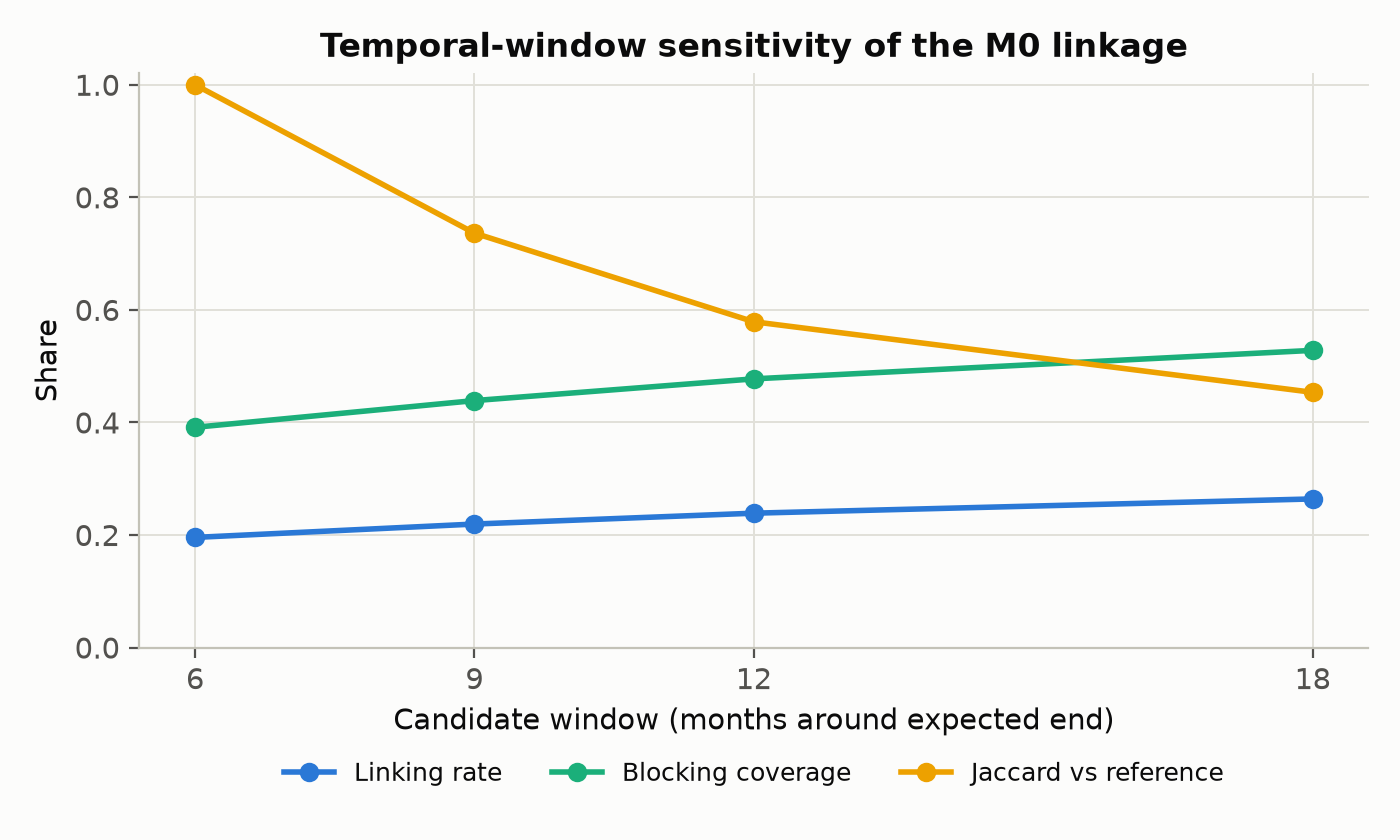
\includegraphics[width=0.8\linewidth]{nb14_window_sensitivity.png}
\caption{Temporal-window sensitivity of the M0 linkage (generated inline by
notebook 14 from \texttt{m6d\_temporal\_window\_sensitivity.csv}): blocking
coverage and linked-event count increase with the window half-width $W$,
while the Jaccard overlap with the 6-month reference link set falls to
0.453 at $W=18$ --- widening the window does not just find \emph{more}
links, it finds \emph{different} ones.}
\label{fig:windowsens}
\end{figure}

\subsection{Duration Leakage and Circularity}
\label{sec:leakage}
Declared/imputed duration enters the pipeline three times: it constructs
$\hat e_i$ (used for blocking), it drives $s_{\text{time}}$ (used for
scoring), and it remains available as a Cox/AFT covariate. This creates a
genuine circularity risk that was tested directly, not assumed away.

\begin{table}[h!]
\centering
\caption{Duration-leakage linkage sensitivity (source:
\texttt{reports/tables/}\newline\texttt{duration\_leakage\_linkage\_sensitivity.csv}).}
\begin{tabular}{p{0.32\textwidth}rrrrr}
\toprule
Definition & Links & Event rate & Jaccard & Status changes & Median gap \\
\midrule
Balanced reference & 618 & 19.6\% & 1.000 & 0 & 37.7 mo \\
No temporal score, reference pool & 618 & 19.6\% & 0.414 & 246 & 42.6 mo \\
Forward 24mo, no duration & 1{,}105 & 35.0\% & 0.064 & 901 & 5.8 mo \\
\bottomrule
\end{tabular}
\end{table}

\begin{table}[h!]
\centering
\caption{Duration-only clustered Cox audit across designs (source:
\texttt{reports/tables/}\newline\texttt{duration\_leakage\_cox\_duration\_effect.csv}); a
single-covariate model isolating $\log(1+d)$'s marginal association.}
\label{tab:leakagecox}
\begin{tabular}{p{0.32\textwidth}rrp{0.22\textwidth}}
\toprule
Design & HR (log dur.) & $p$ (clustered) & Direction \\
\midrule
Balanced reference & 0.620 & $2.1\times10^{-12}$ & Longer duration $\to$ lower hazard \\
No temporal score, reference pool & 0.698 & $3.8\times10^{-5}$ & Longer duration $\to$ lower hazard \\
\textbf{Forward 24mo, no duration} & \textbf{1.344} & \textbf{$9.0\times10^{-8}$} & \textbf{Longer duration $\to$ \emph{higher} hazard} \\
\bottomrule
\end{tabular}
\end{table}
\begin{figure}[h!]
\centering
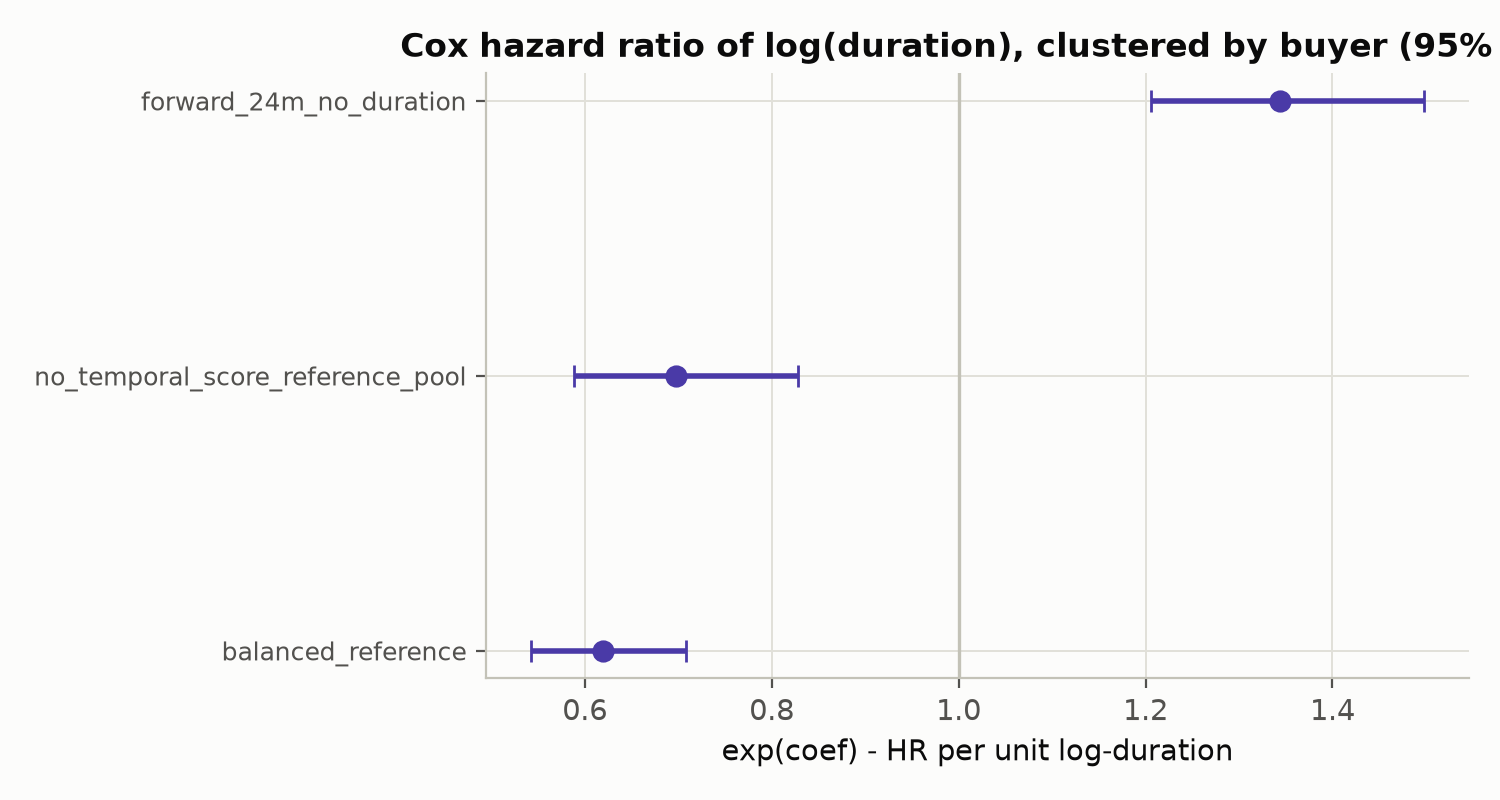
\includegraphics[width=0.8\linewidth]{nb15_cox_duration_hr.png}
\caption{Buyer-clustered hazard ratio of $\log(1+\text{duration})$ with
95\% CI under the three linkage designs (generated inline by notebook 15
from \texttt{duration\_leakage\_cox\_duration\_effect.csv}). The
confidence intervals of the duration-centered designs (HR $<1$) and the
duration-independent forward-window design (HR $>1$) do not overlap ---
the effect's sign is an artifact of the design, not a stable property of
the data.}
\label{fig:leakagehr}
\end{figure}

The sign of the duration effect \textbf{reverses} between the
duration-centered designs (HR $<1$) and the duration-independent forward
window (HR $>1$), as Figure~\ref{fig:leakagehr} makes visually explicit.
This is strong evidence that declared duration should
\emph{not} be interpreted as an independent substantive predictor of
recurrence under the current duration-centered linkage design --- the
apparent effect in Table~\ref{tab:coxnoncpv} is at least partly a
mechanical artifact of how candidates are searched for, not a free-standing
finding about procurement behavior. This is the single highest-priority
caveat in this report.

\subsection{Quantitative Survival-Sensitivity Conclusion}
\label{sec:survival-sensitivity-conclusion}
The quantitative survival conclusion is therefore deliberately modest. Under
the M0 balanced reference, 618 of 3{,}159 sources are linked to a constructed
proxy-recurrence event, with 80.4\% censoring, no reached median survival,
$\hat S(24\text{ months})=0.914$, and RMST$_{60}=53.5$ months. Because the
Kaplan--Meier curve does not cross 50\%, RMST$_{60}$ is the appropriate
descriptive survival summary, not median survival.

The temporal-window sensitivity is moderate in the survival summaries but
large in the underlying event identities. Moving from the 6-month reference
window to an 18-month window raises the proxy-event count from 618 to 834
and the event rate from 19.6\% to 26.4\%, while RMST$_{60}$ falls from
53.5 to 51.4 months. However, the link-set Jaccard overlap falls to 0.453
and 306 source event statuses change. The wider-window curve is therefore
not simply a more complete version of the reference curve; it is based on a
materially different constructed event.

The duration-design checks are more severe. Removing the temporal score
while keeping the reference candidate pool preserves the event count at 618
but changes 246 source event statuses and lowers link-set overlap to
0.414. Replacing the duration-centered design with a forward 24-month
no-duration window produces 1{,}105 events, lowers overlap to 0.064,
changes 901 source event statuses, and reduces the median event time from
37.7 to 5.8 months. In the duration-only Cox audit, the clustered hazard
ratio for $\log(1+\text{duration})$ is 0.620 in the balanced reference and
0.698 in the no-temporal-score reference-pool design, but reverses to 1.344
under the forward 24-month no-duration design.

Finally, among parametric AFT models fit to the balanced reference, the
log-normal model fits better than the Weibull model (AIC 7{,}949.0 vs.
8{,}059.8; concordance 0.725 vs. 0.714). This model comparison is still
conditional on the constructed M0 event and should not be interpreted as
validation of true renewal timing.

In short, the survival results are directionally informative but not
definitive. They should be reported as robustness diagnostics for a
constructed BOAMP proxy-recurrence event, not as stable evidence of verified
renewal timing or as causal evidence about duration.

\subsection{Prediction Calibration (12/24-Month Risk Groups)}
As a bounded, non-operational analogue of a renewal-risk indicator, the
fitted balanced Cox model's predicted risk at 12 and 24 months was grouped
into quintiles and compared to the observed proxy-event rate within each
quintile (\texttt{reports/tables/survival\_predictions\_12\_24m.csv}).

\begin{table}[h!]
\centering
\caption{12-month risk-quintile calibration, balanced variant.}
\begin{tabular}{rrrr}
\toprule
Risk quintile (1=lowest) & $n$ & Mean predicted risk & Observed event rate \\
\midrule
1 & 632 & 0.029 & 0.002 \\
2 & 632 & 0.041 & 0.008 \\
3 & 631 & 0.057 & 0.003 \\
4 & 632 & 0.082 & 0.082 \\
5 (highest) & 632 & 0.190 & 0.275 \\
\bottomrule
\end{tabular}
\end{table}
The highest-risk quintile does show a materially higher observed rate than
the lower quintiles (Figure~\ref{fig:calibration}), so the model carries
\emph{some} ranking signal even in a design known to have duration-leakage
concerns, but calibration is uneven (quintiles 1--3 under-predict relative
to their already-small observed rates; quintile 5 under-predicts the true
rate by roughly 8.5 points).

\begin{figure}[h!]
\centering
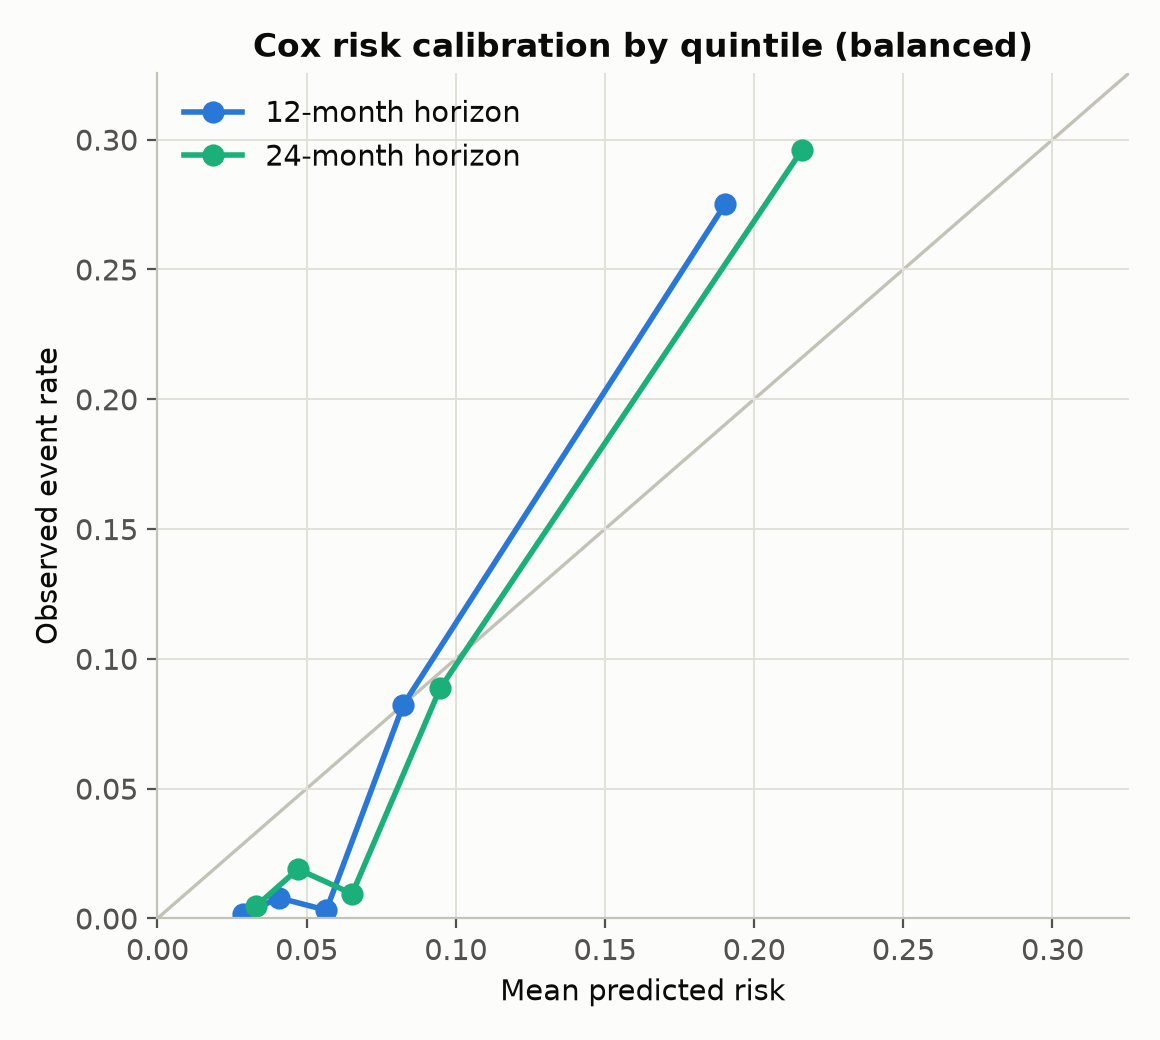
\includegraphics[width=0.75\linewidth]{nb16_calibration_balanced.png}
\caption{Cox risk calibration by predicted-risk quintile, balanced variant,
12- and 24-month horizons (generated inline by notebook 16 from
\texttt{survival\_predictions\_12\_24m.csv}). Bars compare mean predicted
risk to the observed proxy-event rate within each quintile.}
\label{fig:calibration}
\end{figure} \textbf{This is calibration against the constructed BOAMP proxy
event, not against verified legal renewal}, and given
Section~\ref{sec:leakage} it should not be operationalized as a renewal-risk
score without first re-deriving it from a duration-independent linkage
design and validating against manual labels.

\section{Manual-Validation Readiness}
\label{sec:manual}
No completed manual labels exist in this repository, and none were
fabricated for this report. A stratified, unlabeled sample was drawn to
\texttt{reports/tables/manual\_validation\_sample\_unlabeled.csv}, covering
score tiers, margin tiers, selected and non-selected pairs, both buyer-key
types, imputed and observed durations, single- and multi-candidate sources,
and duplicate-candidate cases. The accompanying guide
(\texttt{reports/manual\_validation\_guide.md}) specifies four labels ---
\emph{credible\_renewal}, \emph{likely\_not\_renewal}, \emph{uncertain},
\emph{insufficient\_evidence} --- and instructs reviewers not to infer a
label from the M0 score. At least two independent reviewers and an
adjudication step are recommended before treating labels as observed
validation evidence.

\section{Implementation Status of Every Method}
\label{sec:status}
The user-facing distinction that matters for a handoff is not
``mentioned somewhere'' vs.\ ``not mentioned'' but \emph{how far each
method actually got}. Table~\ref{tab:status} classifies everything this
project has touched, based on executable code and current outputs (the
evidence standard of the credibility audit). Note that
\texttt{audit\_credibility\_implementation\_matrix.csv} records statuses
\emph{as found at the start of the audit}; the table below reflects the
current state, after the audit itself implemented several of the items that
CSV marks ``NOT IMPLEMENTED.''

\begin{table}[h!]
\centering
\caption{Implementation status, current repository state.}
\label{tab:status}
\footnotesize
\begin{tabular}{p{0.30\textwidth}p{0.64\textwidth}}
\toprule
Status & Items \\
\midrule
\textbf{Implemented and verified} (code + current outputs + internal
consistency checks pass) &
Retrieval/parsing/preprocessing/candidate generation/linkage/survival
handoff (34/34 final-audit checks; byte-identical notebook/script outputs);
blocking-coverage, zero-candidate, duplicate-candidate, score-distribution,
and censoring-balance diagnostics; threshold sensitivity; feature ablation;
temporal-window sensitivity ($W\in\{6,9,12,18\}$); duration-leakage audit
(two alternative designs, end-to-end); KM/RMST for all eight event
definitions; clustered Cox, PH and functional-form diagnostics; Weibull and
log-normal AFT; 12/24-month calibration tables. \\
\addlinespace
\textbf{Implemented, still requiring external validation} (runs correctly;
meaning depends on unverified assumptions) &
The M0 event definition itself (no ground truth --- L1); the
Fellegi--Sunter mixture precision/recall estimates (model-based,
conditional on $\Omega$); corruption-recovery rates (strict links are not
ground truth; pool held fixed); every survival covariate effect (proxy
event; duration circularity). \\
\addlinespace
\textbf{Partially implemented} &
Manual validation: the stratified unlabeled sample and annotation guide
exist; no labels have been collected. CPV pairwise log-rank test: attempted
but produced no usable rows in the current run (type mismatch between
numeric-like \texttt{cpv\_division} values and string literals ---
documented defect); descriptive KM/RMST comparison stands in for it. \\
\addlinespace
\textbf{Attempted and explicitly deferred} &
Temporal (train-on-$\leq$2021 / test-on-$>$2021) validation of the Cox
model: attempted for all eight variants; recorded as ``deferred: sparse
high-dimensional Cox design did not yield a stable temporal-validation
fit'' in \texttt{survival\_temporal\_validation.csv}. \\
\addlinespace
\textbf{Evaluated and not adopted} (deliberate, documented) &
Sentence-transformer text embeddings (CPU-impractical at the original
national scale; TF-IDF kept for continuity --- revisiting is a listed next
step); fuzzy buyer-name matching (\texttt{rapidfuzz} is installed but
unused; exact normalized-name matching only); the DILA XML archive as
retrieval source (Opendatasoft API preferred); the stricter
CPV-division-only source definition (1{,}882 sources; kept as a sensitivity
figure, not the headline population). \\
\addlinespace
\textbf{Superseded} &
The entire Run 1 national 2024--2026 corpus and its results (raw files
archived under \texttt{data/raw/boamp\_national\_2024\_2026\_archive/};
no Run 1 output is part of any current result). \\
\addlinespace
\textbf{Proposed, not implemented} &
Weight-perturbation sensitivity grid; placebo/negative controls
(runner-up, date-shifted, cross-buyer); full reblocking corruption study;
one-to-one/capped many-to-one matching sensitivity; full-pipeline or
buyer-level bootstrap; collapsed-CPV Cox redesign; SIRENE-based buyer
reconciliation (would revisit the no-enrichment scope); ``Grand Ouest''
geographic extension. \\
\bottomrule
\end{tabular}
\end{table}

\section{What Can and Cannot Be Concluded}
\label{sec:conclusions}

\textbf{Supported by current evidence:}
\begin{enumerate}
  \item The balanced M0 survival handoff is reproducible and internally
  coherent (Section~\ref{sec:construction}).
  \item Blocking, not scoring, is the dominant restriction on event
  discovery: 60.9\% of eligible sources never enter the candidate universe.
  \item The composite score is internally discriminative: accepted links
  score higher and separate more clearly from runner-ups than the ambient
  candidate pool (Table~\ref{tab:scorepop}).
  \item Text degradation is the strongest single-field corruption stressor
  among the fixed-pool corruption tests.
  \item The event definition is materially sensitive to the temporal-window
  design (Jaccard as low as 0.453 at an 18-month window).
  \item The estimated duration effect on survival hazard is \textbf{not}
  robust to duration-independent linkage redesign --- it reverses sign.
  \item Kaplan--Meier median survival is undefined under every tested event
  definition; RMST at 60 months is the appropriate summary statistic.
\end{enumerate}

\textbf{Not supported by current evidence:}
\begin{enumerate}
  \item This pipeline does not establish verified legal renewal accuracy;
  \texttt{event}=1/0 are proxy-linking outcomes, not adjudicated facts.
  \item The Fellegi--Sunter recall estimate is conditional on the blocked
  candidate universe $\Omega$, not recall over all possible true renewals.
  \item CPV-division segment rankings are not stable across event
  definitions (broad vs.\ strict) and are not confirmatory.
  \item Declared duration should not be reported as an independent
  predictor of recurrence under the current duration-centered design.
  \item The 12/24-month risk-group calibration is calibration to the
  constructed proxy event, not to legal renewal probability, and should not
  be used operationally without further validation.
\end{enumerate}

\section{Reproducibility, Output Files, and Remaining Work}
\label{sec:repro}

\subsection{Reproduction Commands}
The primary workflow is notebook-first (Section~\ref{sec:workflow}):
retrieval stays in scripts, everything downstream runs in the notebooks
with results inline. From the repository root:
\begin{verbatim}
# 1. Retrieval + parsing (external source -> flat interim table): scripts
python3 scripts/download_boamp.py
python3 scripts/parse_boamp.py

# 2. Pipeline: preprocessing, candidate pairs, linkage + survival handoff
jupyter nbconvert --to notebook --execute --inplace \
  notebooks/05_preprocess_boamp_m0.ipynb \
  notebooks/07_build_m0_candidate_pairs.ipynb \
  notebooks/08_run_m0_linkage.ipynb

# 3. Evaluation and analysis notebooks
jupyter nbconvert --to notebook --execute --inplace \
  notebooks/11_eval_m3_fellegi_sunter_mixture.ipynb \
  notebooks/12_eval_m4_corruption_recovery.ipynb \
  notebooks/14_eval_m6d_temporal_window_sensitivity.ipynb \
  notebooks/15_eval_duration_leakage.ipynb \
  notebooks/16_survival_robustness.ipynb
\end{verbatim}
The equivalent headless batch backend (identical logic, byte-identical key
outputs --- Section~\ref{sec:dualimpl}):
\begin{verbatim}
python3 scripts/preprocess_boamp_m0.py
python3 scripts/build_m0_candidate_pairs.py
python3 scripts/run_m0_linkage.py
python3 scripts/eval_m3_fellegi_sunter_mixture.py
python3 scripts/eval_m4_corruption_recovery.py
python3 scripts/eval_m6d_temporal_window_sensitivity.py
python3 scripts/eval_duration_leakage.py
python3 scripts/run_survival_analysis.py
\end{verbatim}
Script-only steps (no notebook counterpart):
\texttt{audit\_current\_project.py} (viewed through notebook 13's
\texttt{RUN\_SCRIPT} toggle), \texttt{eval\_m6a\_threshold\_sensitivity.py},
\texttt{eval\_m6b\_feature\_ablation.py},
\texttt{eval\_m6c\_variant\_km\_robustness.py}, the figure builders
(\texttt{make\_figures.py}, \texttt{make\_evaluation\_figures.py},
\texttt{make\_report\_figures.py} --- figures 01--18; the
\texttt{nb14\_*}/\texttt{nb15\_*}/\texttt{nb16\_*} figures are written by
the notebooks themselves), and the report-assembly helpers
(\texttt{\_build\_schema\_summary.py}, \texttt{\_build\_source\_trace.py},
\texttt{\_build\_final\_audit.py}). Each retrieval script is idempotent
with respect to \texttt{data/raw} (raw files are never overwritten) and
runs are logged to \texttt{reports/run\_logs/run\_log.md}.

\subsection{Key Output Files}
\begin{table}[h!]
\centering
\caption{Primary output files referenced throughout this report.}
\small
\begin{tabular}{p{0.44\textwidth}p{0.5\textwidth}}
\toprule
File & Purpose \\
\midrule
\texttt{data/processed/boamp\_m0\_sources.csv} & M0 digital-scope source population (Section~\ref{sec:pipeline}). \\
\texttt{data/processed/boamp\_m0\_candidate\_pairs.csv} & All blocked/scored candidate pairs, $\Omega$ (Section~\ref{sec:algo}). \\
\texttt{data/processed/boamp\_m0\_links\_broad.csv},\newline\texttt{\ldots\_balanced.csv}, \texttt{\ldots\_strict.csv} & Accepted links per variant. \\
\texttt{data/processed/boamp\_survival\_m0\_balanced.csv} & Official survival handoff (Section~\ref{sec:output}). \\
\texttt{reports/tables/audit\_*.csv} & Credibility-audit tables (Sections~\ref{sec:diagnostics}, \ref{sec:reliability}). \\
\texttt{reports/tables/m3\_*.csv}, \texttt{m4\_*.csv}, \texttt{m6*.csv} & Fellegi--Sunter, corruption-recovery, and sensitivity tables. \\
\texttt{reports/tables/survival\_*.csv} & KM, Cox, AFT, PH-diagnostic, and calibration tables (Sections~\ref{sec:results}--\ref{sec:sensitivity}). \\
\texttt{reports/tables/}\newline\texttt{manual\_validation\_sample\_unlabeled.csv} & Stratified sample awaiting manual review (Section~\ref{sec:manual}). \\
\bottomrule
\end{tabular}
\end{table}

\subsection{Remaining Work}
\begin{itemize}
  \item \textbf{Manual validation} is the single highest-priority next
  step: label the stratified sample (Section~\ref{sec:manual}), with two
  reviewers and adjudication, then compute observed precision/recall.
  \item \textbf{Redesign the duration-independent linkage variant} as a
  candidate primary specification, given the sign-reversal finding in
  Section~\ref{sec:leakage}, rather than treating it only as a sensitivity
  check.
  \item \textbf{Collapse sparse CPV-division dummies} (or apply stronger
  regularization) before re-attempting temporal (train/test) validation of
  the Cox model.
  \item \textbf{Fuzzy or SIRENE-linked buyer-name reconciliation} to reduce
  name-fallback fragmentation (L4) --- while remaining within the project's
  stated no-external-enrichment scope, or explicitly revisiting that scope
  decision.
  \item \textbf{Full reblocking corruption study}, one-to-one/many-to-one
  adjudication of reused candidates, negative controls (runner-up,
  date-shifted, cross-buyer placebos), and full-pipeline or buyer-level
  bootstrap uncertainty all remain deferred, as documented in the
  implementation matrix (\texttt{reports/tables/}\newline\texttt{audit\_credibility\_implementation\_matrix.csv}).
  \item \textbf{Fix the CPV-division log-rank pairwise test} (Section~\ref{sec:results})
  so that a formal significance test, not only descriptive KM/RMST
  comparison, is available for segment-level claims.
  \item If more recurrence signal is later needed, apply the guide's
  ``Grand Ouest extension'' fallback (Brittany/Normandy/Centre-Val de Loire
  departments) --- current volume did not require it for this run.
\end{itemize}

\section*{Conclusion}
The current M0 pipeline is a transparent, fully reproducible, and honestly
audited first linkage design for BOAMP procurement recurrence in Pays de la
Loire's digital/ICT sector. Its balanced survival handoff (3{,}159 sources,
618 proxy-recurrence events) is internally coherent and its composite score
is measurably discriminative. At the same time, low blocking coverage
(39.1\%), non-trivial candidate reuse, real sensitivity to the
temporal-window design, and --- most importantly --- a demonstrated
duration-circularity effect on the estimated survival hazard mean that this
report's survival findings should be read as \textbf{robustness diagnostics
for a constructed BOAMP proxy event}, not as verified renewal probabilities
or causal claims about procurement behavior. The defensible conclusion is
that M0 provides a useful, fully auditable proxy-recurrence signal for
exploratory survival analysis and prioritization, provided any downstream
use explicitly states its conditional nature and treats manual validation
as the next required step before operational deployment.

\begin{thebibliography}{9}
\bibitem{fellegi1969} I.~P. Fellegi and A.~B. Sunter,
``A theory for record linkage,''
\emph{Journal of the American Statistical Association}, 64(328):1183--1210, 1969.
\bibitem{christen2012} P.~Christen,
\emph{Data Matching: Concepts and Techniques for Record Linkage, Entity
Resolution, and Duplicate Detection}. Springer, 2012.
\bibitem{salton1988} G.~Salton and C.~Buckley,
``Term-weighting approaches in automatic text retrieval,''
\emph{Information Processing \& Management}, 24(5):513--523, 1988.
\bibitem{dempster1977} A.~P. Dempster, N.~M. Laird, and D.~B. Rubin,
``Maximum likelihood from incomplete data via the EM algorithm,''
\emph{Journal of the Royal Statistical Society, Series B}, 39(1):1--38, 1977.
\bibitem{winkler1988} W.~E. Winkler,
``Using the EM algorithm for weight computation in the Fellegi--Sunter
model of record linkage,'' \emph{Proceedings of the Section on Survey
Research Methods, American Statistical Association}, 667--671, 1988.
\bibitem{kaplan1958} E.~L. Kaplan and P.~Meier,
``Nonparametric estimation from incomplete observations,''
\emph{Journal of the American Statistical Association}, 53(282):457--481, 1958.
\bibitem{cox1972} D.~R. Cox,
``Regression models and life-tables,''
\emph{Journal of the Royal Statistical Society, Series B}, 34(2):187--220, 1972.
\bibitem{grambsch1994} P.~M. Grambsch and T.~M. Therneau,
``Proportional hazards tests and diagnostics based on weighted residuals,''
\emph{Biometrika}, 81(3):515--526, 1994.
\bibitem{royston2013} P.~Royston and M.~K.~B. Parmar,
``Restricted mean survival time: an alternative to the hazard ratio for the
design and analysis of randomised trials with a time-to-event outcome,''
\emph{BMC Medical Research Methodology}, 13:152, 2013.
\bibitem{brier1950} G.~W. Brier,
``Verification of forecasts expressed in terms of probability,''
\emph{Monthly Weather Review}, 78(1):1--3, 1950.
\bibitem{davidsonpilon2019} C.~Davidson-Pilon,
``lifelines: survival analysis in Python,''
\emph{Journal of Open Source Software}, 4(40):1317, 2019.
\end{thebibliography}

\end{document}
